% !TEX encoding = UTF-8 Unicode
% !TEX TS-program = pdflatex

% toptesti document class
\documentclass[%
    a4paper, % not needed, by default it is a4paper, or also b5paper can be used
    corpo=12pt, % dimension of basic font
    % oneside is generally the way to go
    oneside, % two side optimizes for two-face printing, having chapters open on the right (aka odd numbers), if you don't want blank pages put oneside here
    stile=standard,
    %evenboxes, % not needed, to put supervisors and candidate at the same level
    tipotesi=magistrale,
    numerazioneromana, % roman numbering for appendixes and preambles, up to Table of Contents
    openright, % to force opening on the right for double-sided printing
    cucitura=7mm, % for printing, 7mm should be enough
    %dvipsnames, % for compatibility with xcolor, it does not work
]{toptesi}

%%%%%%%%%%%%%%%%%%%%%%%%%%%%%%%%%%%%%%%%%%%%%%%%%%%%
\usepackage[english]{babel}
\usepackage[utf8]{inputenc}
\usepackage[T1]{fontenc}
\usepackage{lmodern}

\usepackage{hyperref} % must be loaded before glossaries-extra

% bibliography
\usepackage[hyperref=true,backref=true,backend=biber,maxbibnames=9,maxcitenames=2,style=numeric,citestyle=numeric,sorting=none]{biblatex} % hyperref uses links, backref goes back to citations, uses biber as backend, with 9 names at most in bibliography and 2 in citations, citing using numbers, and sorting in citation order
% sorting can be also ydnt for year descending, name, title or ynt for ascending year

\usepackage{adjustbox} % to resize boxes by keeping the same aspect ratio
\usepackage{algorithm} % algorithm environment
\usepackage{algpseudocode} % improved pseudo-code
\usepackage{amsfonts}               %  AMS mathematical fonts
\usepackage{amsmath}
\usepackage{amssymb}                %  AMS mathematical symbols
\usepackage{bm}                     %  black/bold mathematical symbols
\usepackage{booktabs}               %  better tables
\usepackage[labelfont=bf]{caption} % font=footnotesize % to have reduced caption font size
\usepackage{csquotes}
\usepackage{enumitem} %left align the bulleted points
\usepackage{geometry}
%\usepackage{glossaries} % to use acronyms and glossary, it has also glossaries-extra as extension, but commands are different
\usepackage[%
    toc, % puts the link in the ToC
    %record, % to use bib2gls
    abbreviations, % to load abbreviations / acronyms
    nonumberlist, % to avoid printing the numbers of the references in the acronyms page
]{glossaries-extra}
\usepackage{graphicx}               %  post-script images
%\usepackage{iwona} % extra fonts, substitute standard ones
\usepackage{listings} % to insert formatted code
\usepackage{lipsum} % for lorem ipsum text, not needed in the real work
\usepackage{makecell} % to change dimensions of cells, for math cases
\usepackage{mathtools} % for additional commands
\usepackage{mfirstuc} % to have capitalization capabilities
\usepackage[final]{microtype}      % microtypography, final lets latex use it also in bibliography
\usepackage{multirow} % to allow for cells covering more than 1 row in tables
\usepackage{nicefrac}       % compact symbols for 1/2, etc.
%\usepackage[lofdepth,lotdepth]{subfig}
\usepackage{ragged2e} % for justifying text
\usepackage{siunitx} % support for SI units of measurement and number typesetting
\usepackage{subfig}
\usepackage{svg} % for svg support, works only if inkscape is installed, default for Overleaf v2
%\usepackage{subfigure}              %  subfigure compatibility, can be removed if subfig
\usepackage{tabularx} % equal-width columns in tables
\usepackage{textcomp} % extra fonts and symbols
\usepackage{url}            % simple URL typesetting
\usepackage{verbatim} % for extended verbatim support
\usepackage{xcolor} % to define colors and use standard CSS names add dvipsnames as option, but it clashes with xcolor loaded in toptesi, pay attention that if it goes in conflict with tikz/beamer, simply use \documentclass[usenames,dvipsnames]{beamer}, along with other custom options when defining the document class
\usepackage[
    type={CC},
    modifier={by-nc-sa},
    version={4.0},
]{doclicense}

% \setlength\textwidth{7in}
% \setlength\textheight{10in}
% \setlength\oddsidemargin{(\paperwidth-\textwidth)/2 - 1in}
% \setlength\topmargin{(\paperheight-\textheight
% -\headheight-\headsep-\footskip)/2 - 1in}

% this configuration is close to TopTesi in width
% \newgeometry{a4paper,top=3cm,bottom=3cm,left=3cm,right=3cm,%
% heightrounded}
% margins as for libreoffice writer
\newgeometry{top=2cm,bottom=2cm,left=2cm,right=2cm,%
heightrounded}



% how to change Contents to Table of Contents
\addto\captionsenglish{% Replace "english" with the language you use
  \renewcommand{\contentsname}%
    {Table of Contents}%
}

% to change the name of Abbreviations to Acronyms
% not needed if use use entry types and define those
% \renewcommand{\abbreviationsname}{Acronyms}

% to allow line comments in algorithms
\algnewcommand{\LineComment}[1]{\State \(\triangleright\) #1}

% to declare abs and norm
\DeclarePairedDelimiter\abs{\lvert}{\rvert}%
\DeclarePairedDelimiter\norm{\lVert}{\rVert}%

% Swap the definition of \abs* and \norm*, so that \abs
% and \norm resizes the size of the brackets, and the 
% starred version does not.
\makeatletter
\let\oldabs\abs
\def\abs{\@ifstar{\oldabs}{\oldabs*}}
%
\let\oldnorm\norm
\def\norm{\@ifstar{\oldnorm}{\oldnorm*}}
\makeatother


% change this configuration with your info
% if you need fewer or more supervisors you have to change \relatore command by adding or removing lines in the table in toptesi_config
\newcommand{\thesistitle}{Applicazione per simulazione campionato F1}
\newcommand{\thesisuniversitylogo}{images/logo/LogoPolito.jpg} % choose your logo
\newcommand{\thesiscandidatename}{Enrico}
\newcommand{\thesiscandidatesurname}{Ciuffreda}
\newcommand{\thesissupervisoronetitle}{prof.}
\newcommand{\thesissupervisoronename}{Fulvio}
\newcommand{\thesissupervisoronesurname}{Corno}
\newcommand{\thesisdate}{AA. 2020/2021}
\newcommand{\thesiscourse}{Ingegneria Gestionale L-8}
\newcommand{\thesisuniversity}{POLITECNICO DI TORINO}
\newcommand{\thesislevel}{Laurea Triennale } % master or bachelor
\newcommand{\thesiscandidatetext}{Candidato}
\newcommand{\thesissupervisortext}{Relatore}


% fontsize is {size}{spacing}\family
\newcommand {\institutionfont}{\fontsize {22}{30}\scshape}
\newcommand {\divisionfont}{\fontsize {16}{20}\rmfamily}
\newcommand {\pretitlefont}{\fontsize {16}{16}\rmfamily}
\newcommand {\customtitlefont}{\fontsize {21}{28}\scshape}% {iwona}{bx}{n}}
\newcommand {\fixednamesfont}{\fontsize {14}{20}\mdseries}
\newcommand {\namesfont}{\fontsize {14}{20}\bfseries}
\newcommand {\footfont}{\fontsize {15}{18}\rmfamily}


\addbibresource{bibliography.bib}

% to load the glossaries, not needed if using bib2gls
% for glossary entry
% @entry{bird,
%     name={bird},
%     description = {feathered animal},
%     see={[see also]{duck,goose}}
% }

% if this bib file does not work, try using \input{file.tex}
% where all the \newabbreviation commands have been inserted
% containing all the definitions

% Gls to capitalize first letter
% GLS for full uppercase
% for abbreviations also
% glsxtrshort for abbreviation
% similar for long, full, and capital configurations, add pl at the end for plurals
% glsentryshort, long, plural (referred to shorts) must be used when in section titles
% glslink to allow the link but use a different text (as for href)


% if you want to use also description for the abbreviations/acronyms, you should use bib2gls and define all the entries in a bib file, which is incompatible with Overleaf
\newacronym{F1}{F1}{Formula 1}
\newacronym{FIA}{FIA}{Federazione internazionale dell'automobile}
\newacronym{DB}{DB}{Database}
\newacronym{SQL}{SQL}{Structured Query Language}
\newacronym{IDE}{IDE}{Integrated development environment}
\newacronym{UML}{UML}{Unified Modeling Language}
\makeglossaries

\begin{document}

\title{\vspace*{-5mm}\textbf{\thesistitle}\\Summary} % vspace is needed to shift upwards the title
\date{\thesisdate}
\author{\textbf{Candidate}:\\\thesiscandidatename~\thesiscandidatesurname\\
\textbf{Supervisors}:\\\thesissupervisoronetitle~\thesissupervisoronename~\thesissupervisoronesurname\\
\thesissupervisortwotitle~\thesissupervisortwoname~\thesissupervisortwosurname\\
\thesissupervisorthreetitle~\thesissupervisorthreename~\thesissupervisorthreesurname}


\ateneo{\thesisuniversity} % university name
\logosede[5cm]{\thesisuniversitylogo} % logo, square brackets contain the height

\titolo{\thesistitle} % title
%\sottotitolo{Metodo dei satelliti medicei} % subtitle

% place/remove a slash \\ to put the name on the following line or after Master Degree Course
\corsodilaurea{\thesiscourse} % course name


%~251197 % id number is not needed

\candidato{\thesiscandidatename~\textsc{\thesiscandidatesurname}} % candidate

% using tabular we can have more than 1 supervisor under the same column
\relatore{\tabular{@{}l}%
    \xmakefirstuc{\thesissupervisoronetitle}~\thesissupervisoronename~\textsc{\thesissupervisoronesurname}\\[0.4ex]
    \xmakefirstuc{\thesissupervisortwotitle}~\thesissupervisortwoname~\textsc{\thesissupervisortwosurname}\\[0.4ex]
    \xmakefirstuc{\thesissupervisorthreetitle}~\thesissupervisorthreename~\textsc{\thesissupervisorthreesurname}
    \endtabular}
%\terzorelatore{Ciao}

% in this way we have Academic Year without stile=classica, so without lines
%\sedutadilaurea{\textsc{Academic~Year} 2019-2020}% per la laurea magistrale
% for PoliTo there is only month year
\sedutadilaurea{\thesisdate}% per la laurea magistrale
% PhD
%\esamedidottorato{Novembre 1610}
%\ciclodidottorato{XV}

% offset for binding, the smaller the better
%\setbindingcorrection{3mm}



\iflanguage{english}{%
	%\retrofrontespizio{This work is subject to the Creative Commons Licence}

	\CorsoDiLaureaIn{\thesislevel's Degree Course in\space}

	\TesiDiLaurea{\thesislevel's Degree Thesis}

	\InName{in}
	\CandidateName{\xmakefirstuc{\thesiscandidatetext}}% or Candidates
	\AdvisorName{\xmakefirstuc{\thesissupervisortext}}% or Supervisor
	%\TutorName{Tutor}
	%\NomeTutoreAziendale{Internship Tutor}

	%\NomePrimoTomo{First volume}
	%\NomeSecondoTomo{Second Volume}
	%\NomeTerzoTomo{Third Volume}
	%\NomeQuartoTomo{Fourth Volume}
}{}


% front page
% frontespizio can be used for the first page print
% while the custom-made frontpage can be used as hard-cover
% use pdfjoin or pdfseparate to extract or put together the pages if needed
%\frontespizio* % without star the logo is on top
\newgeometry{top=4cm,left=3cm,right=3cm,bottom=4cm,heightrounded}
\begin{titlepage}
\centering
%
{\institutionfont \textbf{\MakeUppercase{\thesisuniversity}} \par}
%
\vspace{\stretch{2}} % changing this number and the others changes the proportion
%
{\divisionfont \textbf{\thesislevel in \thesiscourse} \par}
%
\vspace{\stretch{3}}
%
\includegraphics[width=50mm]{\thesisuniversitylogo}\\
%
\vspace{\stretch{4}}
%
{\divisionfont \textbf{\thesislevel} \par}
%
\vspace{\stretch{3}}
%
{\customtitlefont \textbf{\thesistitle} \par}
%
\vspace{\stretch{10}}
%
\makebox[\textwidth]{\null\hfill\def\arraystretch{2}% % to change the spacing change this number
\begin{minipage}[t]{.375\textwidth}\raggedright
    \begin{adjustbox}{width={\textwidth},totalheight={\textheight},keepaspectratio} % with adjustbox it adapts to the lengths of the names, remove it if you want the same font dimension
    \begin{tabular}[t]{@{}l@{}}
        \fixednamesfont \textbf{\thesissupervisortext} \\
        \namesfont \xmakefirstuc{\thesissupervisoronetitle}~\thesissupervisoronename~\MakeUppercase{\thesissupervisoronesurname}\\
        \namesfont \xmakefirstuc{\thesissupervisortwotitle}~\thesissupervisortwoname~\MakeUppercase{\thesissupervisortwosurname}\\
        \namesfont \xmakefirstuc{\thesissupervisorthreetitle}~\thesissupervisorthreename~\MakeUppercase{\thesissupervisorthreesurname}
    \end{tabular}
    \end{adjustbox}
\end{minipage}
%
\hfill
%
\begin{minipage}[t]{.375\textwidth}\raggedleft
\begin{adjustbox}{width={\textwidth},totalheight={\textheight},keepaspectratio} % with adjustbox it adapts to the lengths of the names, remove it if you want the same font dimension
\begin{tabular}[t]{@{}l@{}}
    \fixednamesfont \textbf{\thesiscandidatetext} \\
    \namesfont \thesiscandidatename~\MakeUppercase{\thesiscandidatesurname}
\end{tabular}
\end{adjustbox}
\end{minipage}\hfill\null}\\
%
\vspace{\stretch{5}}
%
{\footfont \textbf{\thesisdate} \par}
%
\end{titlepage}

\restoregeometry
 % custom frontpage
%\retrofrontespizio
% insert text for the back of the front page
% if you insert any remove the following \paginavuota
% either a blank page or a back is needed to have double-sided printing
% pay attention to leave the space for the page

%\paginavuota % clears a page

\frontmatter

% abstract if needed
% \begin{abstract}
%     % abstract, choose between abstract and summary
% \end{abstract}

% to create blank pages for openright in frontmatter
% use one of the following two methods
% 1) use the following three lines
%\phantom{0} % needed otherwise cleardoublepage does not clean the page because it sees it empty
%\cleardoublepage
%\thispagestyle{empty} % to have empty page, without numbers
% 2) or
\paginavuota % to manually create a blank page

\sommario
% !TEX encoding = UTF-8 Unicode
% !TEX TS-program = pdflatex

\documentclass[%
    12pt, % font size
    oneside, % if it should be done for printing on two-sides or not
    a4paper, % format of paper
    notitlepage, % to remove the title page
]{article}

%%%%%%%%%%%%%%%%%%%%%%%%%%%%%%%%%%%%%%%%%%%%%%%%%%%%
\usepackage[english]{babel}
\usepackage[utf8]{inputenc}
\usepackage[T1]{fontenc}
\usepackage{lmodern}

\usepackage{hyperref} % must be loaded before glossaries-extra

% bibliography
\usepackage[hyperref=true,backref=true,backend=biber,maxbibnames=9,maxcitenames=2,style=numeric,citestyle=numeric,sorting=none]{biblatex} % hyperref uses links, backref goes back to citations, uses biber as backend, with 9 names at most in bibliography and 2 in citations, citing using numbers, and sorting in citation order
% sorting can be also ydnt for year descending, name, title or ynt for ascending year

\usepackage{adjustbox} % to resize boxes by keeping the same aspect ratio
\usepackage{algorithm} % algorithm environment
\usepackage{algpseudocode} % improved pseudo-code
\usepackage{amsfonts}               %  AMS mathematical fonts
\usepackage{amsmath}
\usepackage{amssymb}                %  AMS mathematical symbols
\usepackage{bm}                     %  black/bold mathematical symbols
\usepackage{booktabs}               %  better tables
\usepackage[labelfont=bf]{caption} % font=footnotesize % to have reduced caption font size
\usepackage{csquotes}
\usepackage{enumitem} %left align the bulleted points
\usepackage{geometry}
%\usepackage{glossaries} % to use acronyms and glossary, it has also glossaries-extra as extension, but commands are different
\usepackage[%
    toc, % puts the link in the ToC
    %record, % to use bib2gls
    abbreviations, % to load abbreviations / acronyms
    nonumberlist, % to avoid printing the numbers of the references in the acronyms page
]{glossaries-extra}
\usepackage{graphicx}               %  post-script images
%\usepackage{iwona} % extra fonts, substitute standard ones
\usepackage{listings} % to insert formatted code
\usepackage{lipsum} % for lorem ipsum text, not needed in the real work
\usepackage{makecell} % to change dimensions of cells, for math cases
\usepackage{mathtools} % for additional commands
\usepackage{mfirstuc} % to have capitalization capabilities
\usepackage[final]{microtype}      % microtypography, final lets latex use it also in bibliography
\usepackage{multirow} % to allow for cells covering more than 1 row in tables
\usepackage{nicefrac}       % compact symbols for 1/2, etc.
%\usepackage[lofdepth,lotdepth]{subfig}
\usepackage{ragged2e} % for justifying text
\usepackage{siunitx} % support for SI units of measurement and number typesetting
\usepackage{subfig}
\usepackage{svg} % for svg support, works only if inkscape is installed, default for Overleaf v2
%\usepackage{subfigure}              %  subfigure compatibility, can be removed if subfig
\usepackage{tabularx} % equal-width columns in tables
\usepackage{textcomp} % extra fonts and symbols
\usepackage{url}            % simple URL typesetting
\usepackage{verbatim} % for extended verbatim support
\usepackage{xcolor} % to define colors and use standard CSS names add dvipsnames as option, but it clashes with xcolor loaded in toptesi, pay attention that if it goes in conflict with tikz/beamer, simply use \documentclass[usenames,dvipsnames]{beamer}, along with other custom options when defining the document class
\usepackage[
    type={CC},
    modifier={by-nc-sa},
    version={4.0},
]{doclicense}

%%%%%%%%%%%%%%%%%%%%%%%%%%%%%%%%%%%%%%%%%%%%%%%%%%%%
\usepackage[english]{babel}
\usepackage[utf8]{inputenc}
\usepackage[T1]{fontenc}
\usepackage{lmodern}

\usepackage{hyperref} % must be loaded before glossaries-extra

% bibliography
\usepackage[hyperref=true,backref=true,backend=biber,maxbibnames=9,maxcitenames=2,style=numeric,citestyle=numeric,sorting=none]{biblatex} % hyperref uses links, backref goes back to citations, uses biber as backend, with 9 names at most in bibliography and 2 in citations, citing using numbers, and sorting in citation order
% sorting can be also ydnt for year descending, name, title or ynt for ascending year

\usepackage{adjustbox} % to resize boxes by keeping the same aspect ratio
\usepackage{algorithm} % algorithm environment
\usepackage{algpseudocode} % improved pseudo-code
\usepackage{amsfonts}               %  AMS mathematical fonts
\usepackage{amsmath}
\usepackage{amssymb}                %  AMS mathematical symbols
\usepackage{bm}                     %  black/bold mathematical symbols
\usepackage{booktabs}               %  better tables
\usepackage[labelfont=bf]{caption} % font=footnotesize % to have reduced caption font size
\usepackage{csquotes}
\usepackage{enumitem} %left align the bulleted points
\usepackage{geometry}
%\usepackage{glossaries} % to use acronyms and glossary, it has also glossaries-extra as extension, but commands are different
\usepackage[%
    toc, % puts the link in the ToC
    %record, % to use bib2gls
    abbreviations, % to load abbreviations / acronyms
    nonumberlist, % to avoid printing the numbers of the references in the acronyms page
]{glossaries-extra}
\usepackage{graphicx}               %  post-script images
%\usepackage{iwona} % extra fonts, substitute standard ones
\usepackage{listings} % to insert formatted code
\usepackage{lipsum} % for lorem ipsum text, not needed in the real work
\usepackage{makecell} % to change dimensions of cells, for math cases
\usepackage{mathtools} % for additional commands
\usepackage{mfirstuc} % to have capitalization capabilities
\usepackage[final]{microtype}      % microtypography, final lets latex use it also in bibliography
\usepackage{multirow} % to allow for cells covering more than 1 row in tables
\usepackage{nicefrac}       % compact symbols for 1/2, etc.
%\usepackage[lofdepth,lotdepth]{subfig}
\usepackage{ragged2e} % for justifying text
\usepackage{siunitx} % support for SI units of measurement and number typesetting
\usepackage{subfig}
\usepackage{svg} % for svg support, works only if inkscape is installed, default for Overleaf v2
%\usepackage{subfigure}              %  subfigure compatibility, can be removed if subfig
\usepackage{tabularx} % equal-width columns in tables
\usepackage{textcomp} % extra fonts and symbols
\usepackage{url}            % simple URL typesetting
\usepackage{verbatim} % for extended verbatim support
\usepackage{xcolor} % to define colors and use standard CSS names add dvipsnames as option, but it clashes with xcolor loaded in toptesi, pay attention that if it goes in conflict with tikz/beamer, simply use \documentclass[usenames,dvipsnames]{beamer}, along with other custom options when defining the document class
\usepackage[
    type={CC},
    modifier={by-nc-sa},
    version={4.0},
]{doclicense}

% \setlength\textwidth{7in}
% \setlength\textheight{10in}
% \setlength\oddsidemargin{(\paperwidth-\textwidth)/2 - 1in}
% \setlength\topmargin{(\paperheight-\textheight
% -\headheight-\headsep-\footskip)/2 - 1in}

% this configuration is close to TopTesi in width
% \newgeometry{a4paper,top=3cm,bottom=3cm,left=3cm,right=3cm,%
% heightrounded}
% margins as for libreoffice writer
\newgeometry{top=2cm,bottom=2cm,left=2cm,right=2cm,%
heightrounded}


% \setlength\textwidth{7in}
% \setlength\textheight{10in}
% \setlength\oddsidemargin{(\paperwidth-\textwidth)/2 - 1in}
% \setlength\topmargin{(\paperheight-\textheight
% -\headheight-\headsep-\footskip)/2 - 1in}

% this configuration is close to TopTesi in width
% \newgeometry{a4paper,top=3cm,bottom=3cm,left=3cm,right=3cm,%
% heightrounded}
% margins as for libreoffice writer
\newgeometry{top=2cm,bottom=2cm,left=2cm,right=2cm,%
heightrounded}



% how to change Contents to Table of Contents
\addto\captionsenglish{% Replace "english" with the language you use
  \renewcommand{\contentsname}%
    {Table of Contents}%
}

% to change the name of Abbreviations to Acronyms
% not needed if use use entry types and define those
% \renewcommand{\abbreviationsname}{Acronyms}

% to allow line comments in algorithms
\algnewcommand{\LineComment}[1]{\State \(\triangleright\) #1}

% to declare abs and norm
\DeclarePairedDelimiter\abs{\lvert}{\rvert}%
\DeclarePairedDelimiter\norm{\lVert}{\rVert}%

% Swap the definition of \abs* and \norm*, so that \abs
% and \norm resizes the size of the brackets, and the 
% starred version does not.
\makeatletter
\let\oldabs\abs
\def\abs{\@ifstar{\oldabs}{\oldabs*}}
%
\let\oldnorm\norm
\def\norm{\@ifstar{\oldnorm}{\oldnorm*}}
\makeatother


% change this configuration with your info
% if you need fewer or more supervisors you have to change \relatore command by adding or removing lines in the table in toptesi_config
\newcommand{\thesistitle}{Applicazione per simulazione campionato F1}
\newcommand{\thesisuniversitylogo}{images/logo/LogoPolito.jpg} % choose your logo
\newcommand{\thesiscandidatename}{Enrico}
\newcommand{\thesiscandidatesurname}{Ciuffreda}
\newcommand{\thesissupervisoronetitle}{prof.}
\newcommand{\thesissupervisoronename}{Fulvio}
\newcommand{\thesissupervisoronesurname}{Corno}
\newcommand{\thesisdate}{AA. 2020/2021}
\newcommand{\thesiscourse}{Ingegneria Gestionale L-8}
\newcommand{\thesisuniversity}{POLITECNICO DI TORINO}
\newcommand{\thesislevel}{Laurea Triennale } % master or bachelor
\newcommand{\thesiscandidatetext}{Candidato}
\newcommand{\thesissupervisortext}{Relatore}


\addbibresource{bibliography.bib}

% to load the glossaries, not needed if using bib2gls
% for glossary entry
% @entry{bird,
%     name={bird},
%     description = {feathered animal},
%     see={[see also]{duck,goose}}
% }

% if this bib file does not work, try using \input{file.tex}
% where all the \newabbreviation commands have been inserted
% containing all the definitions

% Gls to capitalize first letter
% GLS for full uppercase
% for abbreviations also
% glsxtrshort for abbreviation
% similar for long, full, and capital configurations, add pl at the end for plurals
% glsentryshort, long, plural (referred to shorts) must be used when in section titles
% glslink to allow the link but use a different text (as for href)


% if you want to use also description for the abbreviations/acronyms, you should use bib2gls and define all the entries in a bib file, which is incompatible with Overleaf
\newacronym{F1}{F1}{Formula 1}
\newacronym{FIA}{FIA}{Federazione internazionale dell'automobile}
\newacronym{DB}{DB}{Database}
\newacronym{SQL}{SQL}{Structured Query Language}
\newacronym{IDE}{IDE}{Integrated development environment}
\newacronym{UML}{UML}{Unified Modeling Language}
\makeglossaries

\begin{document}

\title{\vspace*{-5mm}\textbf{\thesistitle}\\Summary} % vspace is needed to shift upwards the title
\date{\thesisdate}
\author{\textbf{Candidate}:\\\thesiscandidatename~\thesiscandidatesurname\\
\textbf{Supervisors}:\\\thesissupervisoronetitle~\thesissupervisoronename~\thesissupervisoronesurname\\
\thesissupervisortwotitle~\thesissupervisortwoname~\thesissupervisortwosurname\\
\thesissupervisorthreetitle~\thesissupervisorthreename~\thesissupervisorthreesurname}


\title{\vspace*{-5mm}\textbf{\thesistitle}\\Summary} % vspace is needed to shift upwards the title
\date{\thesisdate}
\author{\textbf{Candidate}:\\\thesiscandidatename~\thesiscandidatesurname\\
\textbf{Supervisors}:\\\thesissupervisoronetitle~\thesissupervisoronename~\thesissupervisoronesurname\\
\thesissupervisortwotitle~\thesissupervisortwoname~\thesissupervisortwosurname\\
\thesissupervisorthreetitle~\thesissupervisorthreename~\thesissupervisorthreesurname}


\maketitle

% !TEX encoding = UTF-8 Unicode
% !TEX TS-program = pdflatex

\documentclass[%
    12pt, % font size
    oneside, % if it should be done for printing on two-sides or not
    a4paper, % format of paper
    notitlepage, % to remove the title page
]{article}

%%%%%%%%%%%%%%%%%%%%%%%%%%%%%%%%%%%%%%%%%%%%%%%%%%%%
\usepackage[english]{babel}
\usepackage[utf8]{inputenc}
\usepackage[T1]{fontenc}
\usepackage{lmodern}

\usepackage{hyperref} % must be loaded before glossaries-extra

% bibliography
\usepackage[hyperref=true,backref=true,backend=biber,maxbibnames=9,maxcitenames=2,style=numeric,citestyle=numeric,sorting=none]{biblatex} % hyperref uses links, backref goes back to citations, uses biber as backend, with 9 names at most in bibliography and 2 in citations, citing using numbers, and sorting in citation order
% sorting can be also ydnt for year descending, name, title or ynt for ascending year

\usepackage{adjustbox} % to resize boxes by keeping the same aspect ratio
\usepackage{algorithm} % algorithm environment
\usepackage{algpseudocode} % improved pseudo-code
\usepackage{amsfonts}               %  AMS mathematical fonts
\usepackage{amsmath}
\usepackage{amssymb}                %  AMS mathematical symbols
\usepackage{bm}                     %  black/bold mathematical symbols
\usepackage{booktabs}               %  better tables
\usepackage[labelfont=bf]{caption} % font=footnotesize % to have reduced caption font size
\usepackage{csquotes}
\usepackage{enumitem} %left align the bulleted points
\usepackage{geometry}
%\usepackage{glossaries} % to use acronyms and glossary, it has also glossaries-extra as extension, but commands are different
\usepackage[%
    toc, % puts the link in the ToC
    %record, % to use bib2gls
    abbreviations, % to load abbreviations / acronyms
    nonumberlist, % to avoid printing the numbers of the references in the acronyms page
]{glossaries-extra}
\usepackage{graphicx}               %  post-script images
%\usepackage{iwona} % extra fonts, substitute standard ones
\usepackage{listings} % to insert formatted code
\usepackage{lipsum} % for lorem ipsum text, not needed in the real work
\usepackage{makecell} % to change dimensions of cells, for math cases
\usepackage{mathtools} % for additional commands
\usepackage{mfirstuc} % to have capitalization capabilities
\usepackage[final]{microtype}      % microtypography, final lets latex use it also in bibliography
\usepackage{multirow} % to allow for cells covering more than 1 row in tables
\usepackage{nicefrac}       % compact symbols for 1/2, etc.
%\usepackage[lofdepth,lotdepth]{subfig}
\usepackage{ragged2e} % for justifying text
\usepackage{siunitx} % support for SI units of measurement and number typesetting
\usepackage{subfig}
\usepackage{svg} % for svg support, works only if inkscape is installed, default for Overleaf v2
%\usepackage{subfigure}              %  subfigure compatibility, can be removed if subfig
\usepackage{tabularx} % equal-width columns in tables
\usepackage{textcomp} % extra fonts and symbols
\usepackage{url}            % simple URL typesetting
\usepackage{verbatim} % for extended verbatim support
\usepackage{xcolor} % to define colors and use standard CSS names add dvipsnames as option, but it clashes with xcolor loaded in toptesi, pay attention that if it goes in conflict with tikz/beamer, simply use \documentclass[usenames,dvipsnames]{beamer}, along with other custom options when defining the document class
\usepackage[
    type={CC},
    modifier={by-nc-sa},
    version={4.0},
]{doclicense}

%%%%%%%%%%%%%%%%%%%%%%%%%%%%%%%%%%%%%%%%%%%%%%%%%%%%
\usepackage[english]{babel}
\usepackage[utf8]{inputenc}
\usepackage[T1]{fontenc}
\usepackage{lmodern}

\usepackage{hyperref} % must be loaded before glossaries-extra

% bibliography
\usepackage[hyperref=true,backref=true,backend=biber,maxbibnames=9,maxcitenames=2,style=numeric,citestyle=numeric,sorting=none]{biblatex} % hyperref uses links, backref goes back to citations, uses biber as backend, with 9 names at most in bibliography and 2 in citations, citing using numbers, and sorting in citation order
% sorting can be also ydnt for year descending, name, title or ynt for ascending year

\usepackage{adjustbox} % to resize boxes by keeping the same aspect ratio
\usepackage{algorithm} % algorithm environment
\usepackage{algpseudocode} % improved pseudo-code
\usepackage{amsfonts}               %  AMS mathematical fonts
\usepackage{amsmath}
\usepackage{amssymb}                %  AMS mathematical symbols
\usepackage{bm}                     %  black/bold mathematical symbols
\usepackage{booktabs}               %  better tables
\usepackage[labelfont=bf]{caption} % font=footnotesize % to have reduced caption font size
\usepackage{csquotes}
\usepackage{enumitem} %left align the bulleted points
\usepackage{geometry}
%\usepackage{glossaries} % to use acronyms and glossary, it has also glossaries-extra as extension, but commands are different
\usepackage[%
    toc, % puts the link in the ToC
    %record, % to use bib2gls
    abbreviations, % to load abbreviations / acronyms
    nonumberlist, % to avoid printing the numbers of the references in the acronyms page
]{glossaries-extra}
\usepackage{graphicx}               %  post-script images
%\usepackage{iwona} % extra fonts, substitute standard ones
\usepackage{listings} % to insert formatted code
\usepackage{lipsum} % for lorem ipsum text, not needed in the real work
\usepackage{makecell} % to change dimensions of cells, for math cases
\usepackage{mathtools} % for additional commands
\usepackage{mfirstuc} % to have capitalization capabilities
\usepackage[final]{microtype}      % microtypography, final lets latex use it also in bibliography
\usepackage{multirow} % to allow for cells covering more than 1 row in tables
\usepackage{nicefrac}       % compact symbols for 1/2, etc.
%\usepackage[lofdepth,lotdepth]{subfig}
\usepackage{ragged2e} % for justifying text
\usepackage{siunitx} % support for SI units of measurement and number typesetting
\usepackage{subfig}
\usepackage{svg} % for svg support, works only if inkscape is installed, default for Overleaf v2
%\usepackage{subfigure}              %  subfigure compatibility, can be removed if subfig
\usepackage{tabularx} % equal-width columns in tables
\usepackage{textcomp} % extra fonts and symbols
\usepackage{url}            % simple URL typesetting
\usepackage{verbatim} % for extended verbatim support
\usepackage{xcolor} % to define colors and use standard CSS names add dvipsnames as option, but it clashes with xcolor loaded in toptesi, pay attention that if it goes in conflict with tikz/beamer, simply use \documentclass[usenames,dvipsnames]{beamer}, along with other custom options when defining the document class
\usepackage[
    type={CC},
    modifier={by-nc-sa},
    version={4.0},
]{doclicense}

% \setlength\textwidth{7in}
% \setlength\textheight{10in}
% \setlength\oddsidemargin{(\paperwidth-\textwidth)/2 - 1in}
% \setlength\topmargin{(\paperheight-\textheight
% -\headheight-\headsep-\footskip)/2 - 1in}

% this configuration is close to TopTesi in width
% \newgeometry{a4paper,top=3cm,bottom=3cm,left=3cm,right=3cm,%
% heightrounded}
% margins as for libreoffice writer
\newgeometry{top=2cm,bottom=2cm,left=2cm,right=2cm,%
heightrounded}


% \setlength\textwidth{7in}
% \setlength\textheight{10in}
% \setlength\oddsidemargin{(\paperwidth-\textwidth)/2 - 1in}
% \setlength\topmargin{(\paperheight-\textheight
% -\headheight-\headsep-\footskip)/2 - 1in}

% this configuration is close to TopTesi in width
% \newgeometry{a4paper,top=3cm,bottom=3cm,left=3cm,right=3cm,%
% heightrounded}
% margins as for libreoffice writer
\newgeometry{top=2cm,bottom=2cm,left=2cm,right=2cm,%
heightrounded}



% how to change Contents to Table of Contents
\addto\captionsenglish{% Replace "english" with the language you use
  \renewcommand{\contentsname}%
    {Table of Contents}%
}

% to change the name of Abbreviations to Acronyms
% not needed if use use entry types and define those
% \renewcommand{\abbreviationsname}{Acronyms}

% to allow line comments in algorithms
\algnewcommand{\LineComment}[1]{\State \(\triangleright\) #1}

% to declare abs and norm
\DeclarePairedDelimiter\abs{\lvert}{\rvert}%
\DeclarePairedDelimiter\norm{\lVert}{\rVert}%

% Swap the definition of \abs* and \norm*, so that \abs
% and \norm resizes the size of the brackets, and the 
% starred version does not.
\makeatletter
\let\oldabs\abs
\def\abs{\@ifstar{\oldabs}{\oldabs*}}
%
\let\oldnorm\norm
\def\norm{\@ifstar{\oldnorm}{\oldnorm*}}
\makeatother


% change this configuration with your info
% if you need fewer or more supervisors you have to change \relatore command by adding or removing lines in the table in toptesi_config
\newcommand{\thesistitle}{Applicazione per simulazione campionato F1}
\newcommand{\thesisuniversitylogo}{images/logo/LogoPolito.jpg} % choose your logo
\newcommand{\thesiscandidatename}{Enrico}
\newcommand{\thesiscandidatesurname}{Ciuffreda}
\newcommand{\thesissupervisoronetitle}{prof.}
\newcommand{\thesissupervisoronename}{Fulvio}
\newcommand{\thesissupervisoronesurname}{Corno}
\newcommand{\thesisdate}{AA. 2020/2021}
\newcommand{\thesiscourse}{Ingegneria Gestionale L-8}
\newcommand{\thesisuniversity}{POLITECNICO DI TORINO}
\newcommand{\thesislevel}{Laurea Triennale } % master or bachelor
\newcommand{\thesiscandidatetext}{Candidato}
\newcommand{\thesissupervisortext}{Relatore}


\addbibresource{bibliography.bib}

% to load the glossaries, not needed if using bib2gls
% for glossary entry
% @entry{bird,
%     name={bird},
%     description = {feathered animal},
%     see={[see also]{duck,goose}}
% }

% if this bib file does not work, try using \input{file.tex}
% where all the \newabbreviation commands have been inserted
% containing all the definitions

% Gls to capitalize first letter
% GLS for full uppercase
% for abbreviations also
% glsxtrshort for abbreviation
% similar for long, full, and capital configurations, add pl at the end for plurals
% glsentryshort, long, plural (referred to shorts) must be used when in section titles
% glslink to allow the link but use a different text (as for href)


% if you want to use also description for the abbreviations/acronyms, you should use bib2gls and define all the entries in a bib file, which is incompatible with Overleaf
\newacronym{F1}{F1}{Formula 1}
\newacronym{FIA}{FIA}{Federazione internazionale dell'automobile}
\newacronym{DB}{DB}{Database}
\newacronym{SQL}{SQL}{Structured Query Language}
\newacronym{IDE}{IDE}{Integrated development environment}
\newacronym{UML}{UML}{Unified Modeling Language}
\makeglossaries

\begin{document}

\title{\vspace*{-5mm}\textbf{\thesistitle}\\Summary} % vspace is needed to shift upwards the title
\date{\thesisdate}
\author{\textbf{Candidate}:\\\thesiscandidatename~\thesiscandidatesurname\\
\textbf{Supervisors}:\\\thesissupervisoronetitle~\thesissupervisoronename~\thesissupervisoronesurname\\
\thesissupervisortwotitle~\thesissupervisortwoname~\thesissupervisortwosurname\\
\thesissupervisorthreetitle~\thesissupervisorthreename~\thesissupervisorthreesurname}


\title{\vspace*{-5mm}\textbf{\thesistitle}\\Summary} % vspace is needed to shift upwards the title
\date{\thesisdate}
\author{\textbf{Candidate}:\\\thesiscandidatename~\thesiscandidatesurname\\
\textbf{Supervisors}:\\\thesissupervisoronetitle~\thesissupervisoronename~\thesissupervisoronesurname\\
\thesissupervisortwotitle~\thesissupervisortwoname~\thesissupervisortwosurname\\
\thesissupervisorthreetitle~\thesissupervisorthreename~\thesissupervisorthreesurname}


\maketitle

% !TEX encoding = UTF-8 Unicode
% !TEX TS-program = pdflatex

\documentclass[%
    12pt, % font size
    oneside, % if it should be done for printing on two-sides or not
    a4paper, % format of paper
    notitlepage, % to remove the title page
]{article}

\input{common/packages}

\input{common/summary/packages.tex}

\input{common/package_config}

\input{common/summary/package_config.tex}

\input{common/new_commands}

\input{common/thesis_info.tex}

\addbibresource{bibliography.bib}

% to load the glossaries, not needed if using bib2gls
\input{glossaries.tex}
\makeglossaries

\begin{document}

\input{common/config}

\input{common/summary/config.tex}

\maketitle

\input{content/summary.tex}

\end{document}


\end{document}


\end{document}


\phantom{0}
\cleardoublepage
\thispagestyle{empty}



\paginavuota
\tableofcontents

\listoftables % ToC for tables

\listoffigures % ToC for figures

% actually abbreviation is the name used for acronym in glossaries-extra
% title sets the name
% type tells the type of glossary to print
% style overrides the global style
% here we are printing only abbreviations
% printunsrtglossary if using record, otherwise printglossary is ok
\paginavuota
\printunsrtglossary[style=altlist,title=Acronyms,type=\glsxtrabbrvtype]

% also list of symbols here if needed

% to remove all first use occurrences given the presence of the summary
\glsresetall
% to skip all the first use occurrences, using only short forms
% \glsunsetall


\mainmatter

%\part{Prima Parte} % parts division, not needed
% Chapters always open on a right-side page, i.e. odd numbers, so a blank page is inserted if needed
%\cleardoublepage[empty] % to have a fully blank page
% a blank page appears before the first chapter in some configurations, on the last version it doesn't

% list here all the chapters
\chapter{Proposta di Progetto}
\label{sec:proposta di progetto}

% use [] to set name for ToC
\section[Titolo della proposta]{Titolo della proposta} % ok with fontsize=12pt
Applicazione per simulazione campionato F1
\section[Descrizione del problema proposto ]{Descrizione del problema proposto} % ok with fontsize=12pt
L'applicazione ha come obiettivo quello di simulare un campionato di Formula 1 per assegnare il titolo iridato al pilota che ha guadagnato più punti all'interno delle gare previste e per assegnare il cosiddetto campionato costruttori, ovvero il premio alla scuderia che ha guadagnato più punti. La simulazione sarà basata sui dati reali dei vari anni e quindi sulle capacità dei vari piloti e dalle performance delle macchine delle varie scuderie. La simulazione verrà effettuata gara per gara.
\section[Descrizione della rilevanza gestionale del problema]{Descrizione della rilevanza gestionale del problema} % ok with fontsize=12pt
L’applicazione può avere diversi scopi in base al ruolo dell’utente. Nel caso in cui l’utente faccia parte di una scuderia allora l’applicazione servirebbe per simulare il campionato sostituendo un pilota con uno nuovo o scambiando due piloti di due scuderie diverse o per simulare il campionato dopo aver investito un extra nella scuderia e quindi vedendo la propria macchina migliorata. Nel caso in cui l’utente sia un semplice fruitore allora potrebbe usare l’applicazione per raccogliere dati per quanto concerne il settore delle scommesse.
\section[Descrizione dei data-set per la valutazione]{Descrizione dei data-set per la valutazione} % ok with fontsize=12pt
L’applicazione fa uso di un solo dataset disponibile all’indirizzo \\\url{http://ergast.com/mrd/db}, in cui sono presenti i dati di tutti i circuiti, di tutti i piloti e di tutti i risultati delle varie qualifiche e gare. Il database è rilasciato con licenza “Attribution-NonCommercial-ShareAlike 3.0 Unported Licence”. Al dataset viene aggiunto una tabella contenente la valutazione di ogni pilota. Questi ultimi dati vengono presi direttamente dal gioco “F12020” licenziato dalla FIA e prodotto da Codemaster e una tabella contenente i vari importi degli investimenti fatti da ciascuna scuderia nel corso del 2019 ricavati dai budget pubblici rilasciati dalle diverse scuderie.
\section[Descrizione preliminare degli algoritmi coinvolti]{Descrizione preliminare degli algoritmi coinvolti} % ok with fontsize=12pt
Il principale algoritmo coinvolto è un algoritmo simulativo a eventi discreti. Le tipologie di eventi sono: Qualifica, Gara, Incidente, Sorpasso. I tempi della qualifica si baseranno sui dati degli anni precedenti sullo stesso circuito. Poiché sono presenti solo le valutazioni dei piloti dell’anno in corso viene preso il giro più veloce e vengono aggiunti o sottratti secondi in base alla differenza di valutazione del pilota, alla valutazione della macchina e ad un fattore casuale così da poter formare la griglia di partenza per la gara. L’evento gara permetterà di simulare l’intera gara e quindi i diversi giri, nei quali i piloti potranno sorpassare le vetture che li precedono attraverso l’evento sorpasso che si attiverà quando i due piloti sono ad una distanza prefissata. L’evento sorpasso avrà una probabilità di riuscita che dipende dall’abilità del pilota, alla valutazione della macchina, ad un fattore casuale e alla presenza della scia. Al termine della gara verranno assegnati i punti ai piloti in base al loro posizionamento e una volta finite le gare verrà assegnato il premio per il pilota con più punti e la scuderia con più punti.
Descrizione preliminare delle funzionalità previste per l’applicazione software
L’applicazione sarà divisa in due parti. 
La prima parte presenterà un menù a tendina dal quale è possibile scegliere se scambiare un pilota di una scuderia con un altro pilota di un’altra scuderia, scambiare un pilota di una scuderia con un pilota esterno al circus e in questo caso il nome potrà essere impostato direttamente dall’utente così come la valutazione del pilota che potrà essere generata in maniera casuale o inserita dall’utente. Una terza opzione del menù permetterà di inserire l’importo (in milioni di euro) da investire per aumentare la qualità della macchina. L’ultima impostazione che l’utente può inserire la possibilità di pioggia durante le qualifiche e durante le gara. Un bottone “SIMULA” permetterà all’utente di iniziare la simulazione.
La seconda parte invece presenterà i risultati relativi alla simulazione. I risultati saranno visualizzati in tabella e con un menù a tendina sarà possibile passare dalla classifica piloti alla classifica costruttori. Sarà inoltre possibile visualizzare i risultati di ogni gara. Un bottone “NUOVA SIMULAZIONE” permetterà all’utente di tornare alla prima sezione e ripristinare le varie classifiche.


\chapter{Descrizione dettagliata del problema}
\label{sec:descrizione dettagliata del problema}


% use [] to set name for ToC
\section[Campionato di F1]{Campionato di F1} % ok with fontsize=12pt
Il campionato di F1 è un campionato mondiale automobilistico organizzato dalla FIA. Il campionato è composto da un numero variabile di gare che possono essere disputate nei vari Paesi del Mondo. In genere una settimana in cui vi è la gara è composta da 3 parti: 
\begin{itemize}
\item \textbf{Prove libere} (generalmente svolte il venerdì), dove vengono provati i vari setup per le macchine;
\item \textbf{Qualifiche} (generalmente svolte il sabato), dove i piloti si qualificano alla gara e cercano di avere il miglior posto possibile in griglia di partenza per la gara;
\item \textbf{Gara} (generalmente svolta la domenica).
\end{itemize}
Al termine del campionato vengono assegnati due tipi diversi di titoli: il \textbf{Premio Costruttore}, assegnato alla scuderia che ha totalizzato più punti nel corso del campionato e il  \textbf{Premio pilota}, assegnato al pilota che ha totalizzato più punti nel corso del campionato  .\\
A seguito della pandemia da Covid-19, il campionato di F1 2020 è stato caratterizzato da un numero ridotto di gare, dall'assenza di alcuni piloti in determinate gare e dall'introduzione di un sistema che ha come obiettivo quello di minimizzare il gap tra le varie scuderie limitando gli investimenti delle scuderie e limitando il numero di possibili sostituzioni nei pezzi che compongono la vettura.

\section[Obiettivi]{Obiettivi} % ok with fontsize=12pt
L'applicazione ha vari obiettivi che però possono essere raggruppati in due insiemi. Da una parte abbiamo gli obiettivi finalizzati ad aiutare una scuderia nelle scelte effettuate ad inizio anno, come possono essere quelle della scelta del pilota o della scelta della quantità di investimenti da effettuare. Inoltre poichè l'applicazione simula e riporta la classifica di  ogni gara, una scuderia può anche cercare di migliorare le prestazioni in quella determinata gara. D'altra parte abbiamo invece, gli obiettivi finalizzati ad un calcolo probabilistico della vittoria del titolo piloti, del titolo costrutturi e della griglia di partenza e della classifica finale di ogni gara; questi risultati, ottenuti dalla simulazione ripetuta più volte, possono essere ad esempio una base di partenza per calcolare la quotazione di ogni evento da parte dei bookmakers.
\section[Criticità]{Criticità} % ok with fontsize=12pt
L'applicazione presenta varie criticità dovute sopratutto all'impossibilità di recuperare qualsiasi tipo di dato relativo alle varie vetture poichè questi dati rimangono segreti all'interno delle varie scuderie e non vengono pubblicati. Non è quindi possibile analizzare le varie componenti e conseguentemente non è possibile nemmeno quantificare le prestazioni come ad esempio la velocità massima o la velocità in curva.\\
Un ulteriore criticità è rappresentata dall'irrealistica, ma efficace a livello simulativo, semplificazione dell'abilità di un pilota. Infatti l'applicazione non tiene conto delle varie qualità che un pilota può avere, un esempio potrebbe essere il caso in cui un pilota potrebbe schivare un altro pilota e quindi non effettuare un incidente grazie alla sua destrezza mentre nella stessa situazione un altro pilota potrebbe essere coinvolto poichè i suoi riflessi non sono così eccellenti.\\
Un ulteriore criticità è quella di non implementare una strategia di scuderia per ogni gara ma utilizzare una strategia fornita dai dati degli anni passati.\\
Le ultime due criticità sono rappresentate dal consumo degli pneumatici e dalla temperatura e dallo stato dell'asfalto.


\chapter{Dataset}
\label{sec:dataset}


% use [] to set name for ToC
\section[Informazioni introduttive]{Informazioni introduttive} % ok with fontsize=12pt
I dati utilizzati sono divisibili in tre diverse categorie:
\begin{itemize}
\item  Dati dei circuiti, dei piloti e delle scuderie e relative prestazioni in tutte le gare;
\item  Dati utlizzati per quantificare il valore tecnico di ciascun pilota;
\item  Dati riguardanti gli investimenti fatti dalle scuderie nel 2020.
\end{itemize}
Il software è stato realizzato per poter essere aggiornato con le prestazioni dei piloti e delle scuderie negli anni successivi.\\
A scopo di esempio e per testare le funzionalità dell'applicazione sono stati utilizzati i dati riguardanti tutte le stagioni fino alla fine del campionato di F1 del 2020. Tali dati sono stati estratti al seguente indirizzo: \href{http://ergast.com/mrd/db/}{http://ergast.com/mrd/db/}. Allo script sql, rilasciato con licenza Attribution-NonCommercial-ShareAlike 3.0 Unported Licence, è poi necessario aggiungere uno script sql che comprende una tabella per assegnare i punteggi ad ogni pilota ed una tabella che riporta gli importi spese dalle scuderie.\\
Nella directory "db" è possibile trovare un file in formato sql che contiene al suo interno sia i dati delle prestazioni sia i dati riguardanti il punteggio dei piloti e le spese dei vari team; è inoltre disponibile anche il solo esempio dei punteggi e delle spese ed è anche disponibile un altro file utile se si ha già un database chiamato "F1".

\begin{figure}[h]
\centering
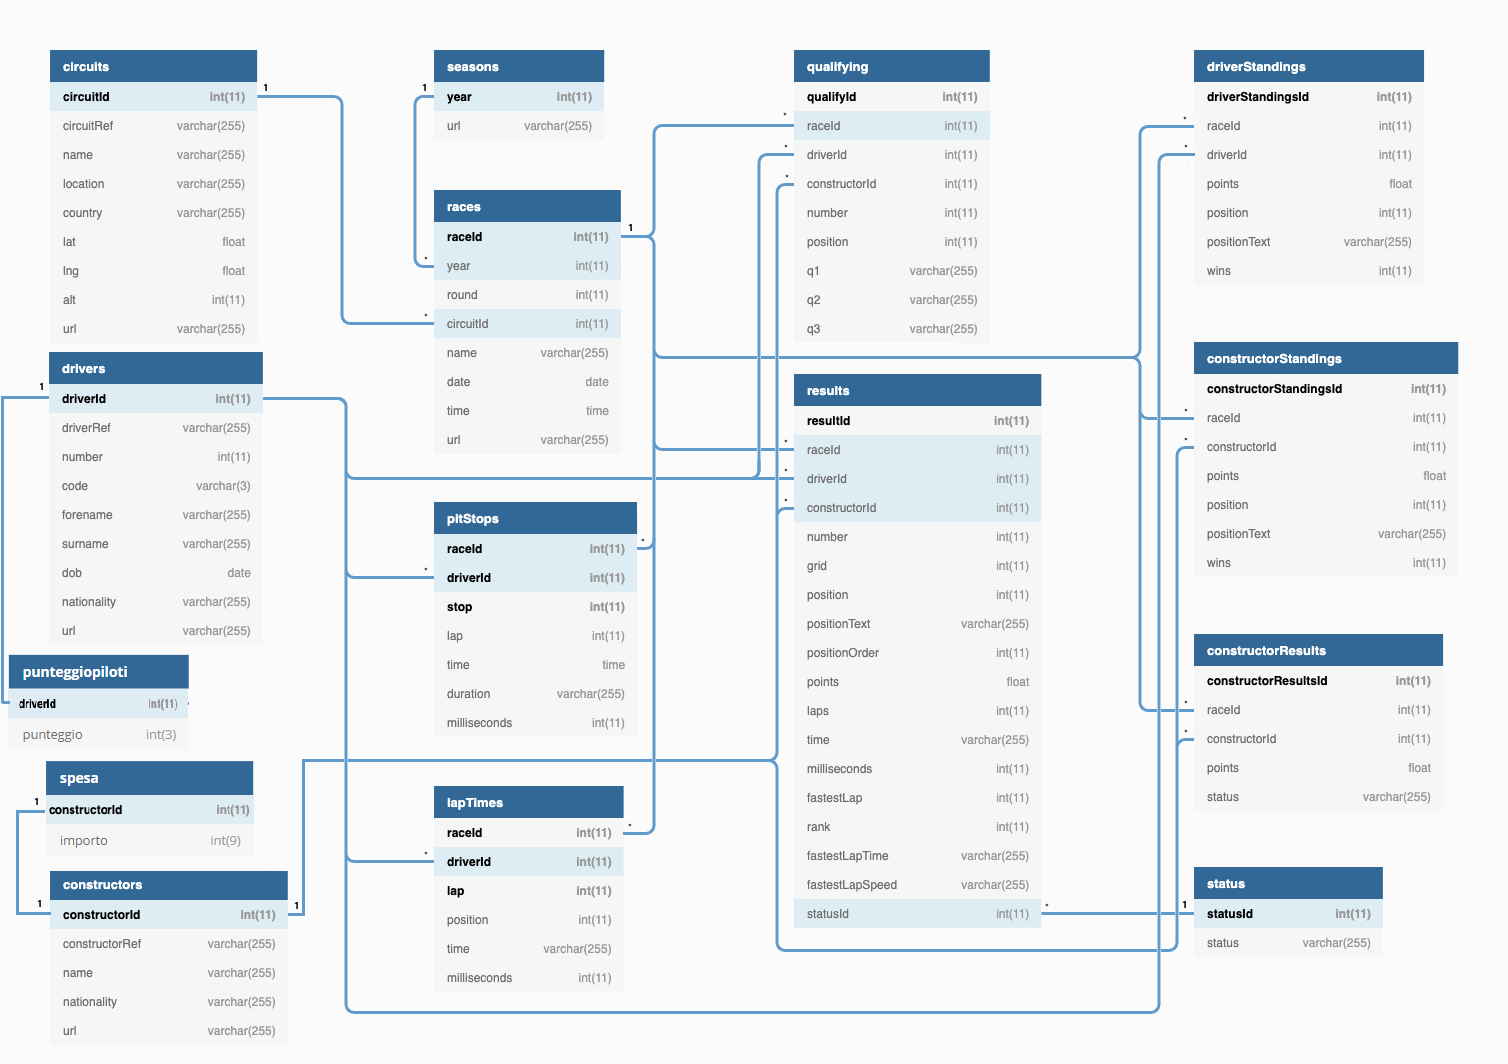
\includegraphics[width=1\linewidth]{images/Diagramma ER.png}
\caption{Diagramma ER}
\label{fig:Diagramma ER}
\end{figure}

\section[Descrizione delle tabelle]{Descrizione delle tabelle}
\subsection{tabella circuits}% ok with fontsize=12pt
\begin{enumerate}
    \item\textbf{ circuitid}: codice identificativo del circuito;
    \item \textbf{circuitRef}: stringa identificativa per il circuito;
    \item \textbf{name}: nome del circuito;
    \item \textbf{location}: città in cui si trova il circuito;
    \item \textbf{country}: Paese in cui si trova il circuito;
    \item \textbf{lat}: latitudine del punto in cui si trova il circuito;
    \item \textbf{lng}: longitudine del punto in cui si trova il circuito;
    \item \textbf{alt};
    \item \textbf{url}: link wikipedia del circuito;
\end{enumerate}
\subsection{tabella drivers}% ok with fontsize=12pt
\begin{enumerate}
    \item \textbf{driversid}: codice identificativo del pilota;
    \item \textbf{driverRef}: stringa identificativa per il pilota (generalmente uguale al surname);
    \item \textbf{number}: numero utilizzato dal pilota;
    \item \textbf{code}: stringa di 3 caratteri per identificare il pilota;
    \item \textbf{forename}: nome del pilota;
    \item \textbf{surname}: cognome del pilota;
    \item \textbf{dob}:data di nascita del pilota;
    \item \textbf{nationality}: Paese del pilota;
    \item \textbf{url}: link wikipedia del pilota;
\end{enumerate}
\subsection{tabella constructors}% ok with fontsize=12pt
\begin{enumerate}
    \item \textbf{constructorId}: codice identificativo della scuderia;
    \item \textbf{constructorRef}: stringa identificativa per la scuderia (generalmente uguale al name);
    \item \textbf{nome}: nome della scuderia;
 \textbf{nationality}: Paese della scuderia;
    \item \textbf{url}: link wikipedia della scuderia;
\end{enumerate}
\subsection{tabella races}% ok with fontsize=12pt
\begin{enumerate}
    \item \textbf{raceid}: codice identificativo della gara;
    \item \textbf{year}: anno di svolgimento della gara;
    \item \textbf{round}: numero progressivo annuale;
    \item \textbf{circuitid}: codice identificativo del circuito;
    \item \textbf{name}: nome che viene dato alla gara;
    \item \textbf{data}: data in cui si svolge la gara;
    \item \textbf{time}: orario in cui si svolge la gara;
    \item \textbf{url}: link wikipedia della gara;
\end{enumerate}
\subsection{tabella pitStops}% ok with fontsize=12pt
\begin{enumerate}
    \item \textbf{raceid}: codice identificativo della gara;
    \item \textbf{driverid}: codice identificativo;
    \item \textbf{stop}: numero progressivo di stop per ogni pilota per ogni gara;
    \item \textbf{lap}: giro in cui è stato effettuato il pitstop;
    \item \textbf{time}: ora in cui è stato effettuato il pitstop;
    \item \textbf{duration}: durata del pitstop;
    \item \textbf{milliseconds}: durata del pitsop in millisecondi;
\end{enumerate}
\subsection{tabella lapTimes}% ok with fontsize=12pt
\begin{enumerate}
    \item \textbf{raceid}: codice identificativo della gara;
    \item \textbf{driverid}: codice identificativo del pilota;
    \item \textbf{lap}: giro in cui è stato effettuato il pitstop;
    \item \textbf{position}: posizione in cui si trova il pilota all'inizio del giro;
    \item \textbf{time}: durata del giro;
    \item \textbf{milliseconds}: durata del pitsop in millisecondi;
\end{enumerate}
\subsection{tabella qualifying}% ok with fontsize=12pt
\begin{enumerate}
    \item qualifyid: codice identificativo della qualifica, diverso per ogni gara e per ogni pilota;
    \item \textbf{raceid}: codice identificativo della gara;
    \item \textbf{driverid}: codice identificativo del pilota;
    \item \textbf{constructorid}: codice identificativo della scuderia;
    \item \textbf{number}: numero del pilota;
    \item \textbf{position}: posizione guadagnata dal pilota in griglia di partenza;
    \item \textbf{q1}: durata del miglior giro in q1;
    \item \textbf{q2}: durata del miglior giro in q2;
    \item \textbf{q3}: durata del miglior giro in q3;
\end{enumerate}
\subsection{tabella results}% ok with fontsize=12pt
\begin{enumerate}
    \item \textbf{resultid}: codice identificativo del risultato di una gara;
    \item \textbf{raceid}: codice identificativo della gara;
    \item \textbf{driverid}: codice identificativo del pilota;
    \item \textbf{constructorid}: codice identificativo della scuderia;
    \item \textbf{number}: numero del pilota;
    \item \textbf{grid}: posizione iniziale del pilota;
    \item \textbf{position}: posizione finale del pilota (null per piloti che si sono ritirati durante la gara);
    \item \textbf{positionText}: viene riportato sotto forma di stringa la posizione o il motivo di ritiro;
    \item \textbf{positionOrder}: posizione finale del pilota;
    \item \textbf{points}: punti guadagnati in gara;
    \item \textbf{laps}: numero di giri compiuti;
    \item \textbf{time}: durata della gara;
    \item \textbf{milliseconds}: durata della gara in millisecondi;
    \item \textbf{fastestLap}: indicazione del giro in cui è stato fatto il miglior tempo;
    \item \textbf{rank}: posizione rispetto agli altri piloti per quanto riguarda i giri veloci;
    \item \textbf{fastestLapTime}: durata in millisecondi del miglior giro del pilota;
    \item \textbf{fastestLapSpeed}: velocità media di percorrenza del giro veloce;
    \item \textbf{statusId} : numero che corrisponde allo status del pilota ( nella tabella status viene indicato a cosa corrisponde ogni numero);
\end{enumerate}
\subsection{tabella driverStandings}% ok with fontsize=12pt
\begin{enumerate}
    \item \textbf{driverStandingsid}: codice identificativo del risultato del pilota in una gara;
    \item \textbf{raceid}: codice identificativo della gara;
    \item \textbf{driverid}: codice identificativo del pilota;
    \item \textbf{points}: punti guadagnati in gara;
   \item \textbf{position}: posizione finale del pilota (null per piloti che si sono ritirati durante la gara);
    \item \textbf{positionText}: viene riportato sotto forma di stringa la posizione o il motivo di ritiro;
    \item \textbf{wins}: valore binario per indicare la vittoria o no del pilota;
\end{enumerate}
\subsection{tabella constructorStandings}% ok with fontsize=12pt
\begin{enumerate}
    \item \textbf{constructorStandingsid}: codice identificativo del risultato della scuderia in una gara;
    \item \textbf{raceid}: codice identificativo della gara;
    \item \textbf{constructorid}: codice identificativo della scuderia;
    \item \textbf{points}: punti guadagnati in gara;
   \item \textbf{position}: posizione finale della scuderia;
    \item \textbf{positionText}: viene riportato sotto forma di stringa la posizione o il motivo di ritiro;
    \item \textbf{wins}: valore binario per indicare la vittoria o no della scuderia;
\end{enumerate}
\subsection{tabella constructorResults}% ok with fontsize=12pt
\begin{enumerate}
    \item \textbf{constructorResultsid}: codice identificativo del risultato della scuderia in una gara;
    \item \textbf{raceid}: codice identificativo della gara;
    \item \textbf{constructorid}: codice identificativo della scuderia;
    \item \textbf{points}: punti guadagnati in gara;
    \item \textbf{status}: variabile per indicare il motivo di ritiro della scuderia;
\end{enumerate}

\chapter{Strutture dati e algoritmi utilizzati}
\label{sec:strutture dati e algoritmi utilizzati}

\begin{table}[]
    \centering
    \setcellgapes{3pt}
    \makegapedcells
    \begin{tabular}{|c|c|c|}
    \hline
    \textbf{Nome del package} & \textbf{Numero di classi} & \textbf{Descrizione}\\ \hline
    DB & 3 & Collegamento al database\\ \hline
    Model & 14 & Algoritmi\\ \hline
    SimulazioneF1 & 5 & Controller interfaccia grafica\\ \hline
    \end{tabular}
    \caption{schema dei package}
    \label{tab:schema dei package}
\end{table}
% use [] to set name for ToC
\section[Struttura del progetto]{Struttura del progetto} % ok with fontsize=12pt
L'applicazione, scritta in linguaggio Java, segue il pattern  pattern MVC(Model View Controller), quindi dividendo la struttura software in 3 parti principali: model, view e controller. Inoltre l'applicazione sfrutta il pattern DAO (Database Access Object), che permette di accedere ai dati sul database, basandosi sugli input dell'utente (ad esempio il numero di gare) e ricavando informazioni poi processate dal Model.\\
Il progetto dell'applicazione è disponibile nel repository Github al seguente link: \href{https://github.com/TdP-prove-finali/CiuffredaEnrico}{https://github.com/TdP-prove-finali/CiuffredaEnrico}.\\
Il progetto si compone di 3 package:
\begin{itemize}

    \item\textbf{ DB}: contiene tutte le classi utili a: collegarsi al database ed estrarne i dati seguendo il pattern DAO;
    \item \textbf{Model}: contiene tutte le classi utilizzati per memorizzare i dati, tutte le classi necessarie per la memorizzazione dei dati, le classi utilizzate per stampare dei dati e le classi utilizzate per la generazione degli eventi gara e qualifica e quindi per la loro simulazione;
    \item \textbf{SimulazioneF1}: contiene tutte le classi per gestire l'interfaccia grafica dell'applicazione. Al suo interno è disponibile una classe \textit{Controller} per ognuna delle due scene, la prima che permette al pilota di impostare alcuni parametri nella simulazione e la seconda utilizzata per stampare a schermo i risultati ottenuti dalla simulazione. La classe \textit{CambiaScena} è invece utlizzata per passare dalla prima scena alla seconda e viceversa.
\end{itemize}
\section[Software utilizzati]{Software utilizzati} % ok with fontsize=12pt
L'applicazione è stata realizzata tramite l'IDE Ecplise. Per la realizzazione di parte dell'interfaccia grafica è stato utilizzato il software SceneBuilder.\\
Il DBMS utilizzato è MariaDB con interfaccia grafica HeidiSQL.
\begin{figure}[h]
\centering
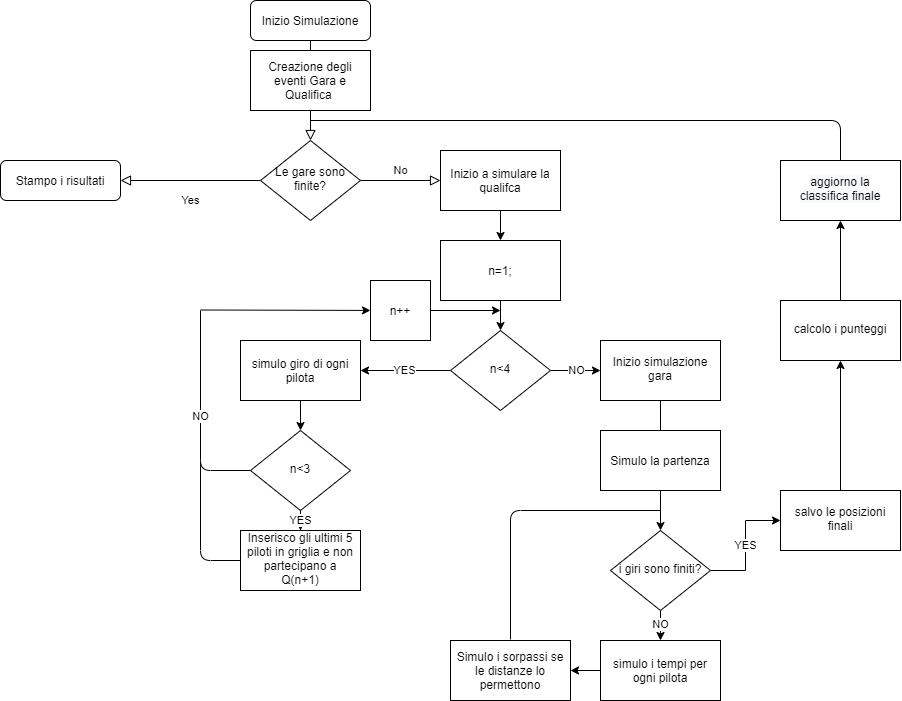
\includegraphics[width=1\linewidth]{images/Flowchart simulazione.png}
\caption{Flowchart simulazione}
\label{fig:Flowchart simulazione}
\end{figure}

\section[Algoritmi]{Algoritmi} % ok with fontsize=12pt
L'applicazione presenta alcuni algoritmi fondamentali.
\subsection{Algoritmo di modifica dati in base a parametri scelti dall'utente}
Lo scopo di questo algoritmo, contenuto nella classe \textit{Model}, è quello di poter permettere all'utente di influenzare la simulazione attraverso 3 procedure: 
\begin{itemize}
\item Sostituzione di un pilota presente in lista con un pilota con dati introdotti dall'utente;
\item Scambio di scuderia tra due piloti. Lo scambio prevede che i tempi dei piloti siano diminuiti o aumentati in base alla differenza di punteggio assegnato alle due diverse macchine;
\item Miglioramento di una scuderia attraverso l'investimento di un numero, inserito dall'utente, di milioni di euro. L'investimento fa sì che i tempi dei giri di gara e qualifica dei due piloti della scuderia vengano diminuiti in base al miglioramento apportato alla macchina utilizzando questi nuovi fondi.
\end{itemize}
\subsection{Algoritmo di generazione eventi}
Lo scopo di questo algoritmo, contenuto nella classe \textit{Simulatore}, è quello di generare gli eventi su cui effettuare la simulazione. Come possiamo notare dalla classe \textit{Evento}, abbiamo due tipi di eventi che possono essere creati: evento QUALIFICA ed evento GARA; questi eventi vengono generati insieme poichè ad ogni gara deve corrispondere una ed una sola qualifica ed ad ogni qualifica deve corrispondere una ed una sola gara. Questo algoritmo utilizza i dati proveniente dal database per scegliere quali sono i circuiti in cui i piloti dovranno gareggiare.
\subsection{Algoritmo di simulazione della qualifica}
Lo scopo di questo algoritmo, contenuto nella classe \textit{SimulatoreQualifica}, è quello di riuscire a simulare l'intera qualifica e quindi di poter generare una griglia di partenza per la gara del giorno successivo. L'algoritmo può essere diviso in diverse parti:
\begin{itemize}

    \item \textbf{Simulazione del giro}: in base ai risultati ottenuti da un pilota nelle qualifiche degli anni precedenti viene stimato un tempo di percorrenza del giro. Questo tempo viene poi diminuito o aumentato in base ad una variabile casuale (ogni valore viene aumentato in percentuale se durante la qualifica piove);
    \item \textbf{Calcolo del tempo impiegato per un giro}: nel caso in cui il pilota, del quale si vuole calcolare il tempo di percorrenza del giro, non abbia mai corso su quel circuito allora il tempo del giro viene calcolato attraverso un algoritmo basato sulla differenza di abilità tra il pilota e un altro pilota estratto da quelli presenti in lista e sulla differenza del punteggio assegnato alla macchina del pilota e dello stesso pilota scelto come confronto. Questo tempo viene poi diminuito o aumentato in base ad una variabile casuale (ogni valore viene aumentato in percentuale se durante la qualifica piove);
    \item \textbf{Sostituzione piloti infortunati e incidenti}: Ad ogni giro compiuto da un pilota è presente una probabilità che esso faccia un incidente. L'incidente può essere di 3 entità: 
    \begin{enumerate}
    \item il pilota rimane illeso e può partecipare alla gara ma parte nell'ultima posizione disponibile. Nel caso l'incidente avvenga in Q1 la posizione è uguale all'ultimo posto, in Q2 equivale al quindicesimo posto e in Q3 equivale al decimo posto;
    \item il pilota dovrà saltare la gara del giorno dopo;
    \item il pilota dovrà saltare la gara del giorno dopo e un'ulteriore gara.
    \end{enumerate}
    Nei casi in cui un pilota è infortunato viene sostiuito da un altro pilota che potrà ottenere punti per la scuderia e punti per sè stesso ma non per il pilota che viene sostiuito.
    \item \textbf{Aggiornamento griglia di partenza}: Il sistema knock-out, utilizzato in F1, prevede 3 step. Al primo step partecipano tutti i piloti. Alla fine dei primi due step vengono eliminati 5 piloti e le loro posizioni in griglia di partenza vengono calcolate in base ai loro tempi. Nell'ultimo step vengono poi assegnati le prime dieci posizione in base allo stesso criterio.
\end{itemize}
\subsection{Algoritmo di simulazione della gara}
Lo scopo di questo algoritmo, contenuto nella classe \textit{SimulatoreGara}, è quello di riuscire a simulare l'intera gara e quindi di poter assegnare i punti in base alla posizione finale del pilota. L'algoritmo può essere diviso in diverse parti:
\begin{itemize}

    \item \textbf{Simulazione del giro}: in base ai risultati ottenuti da un pilota nelle gare degli anni precedenti sullo stesso circuito viene stimato un tempo di percorrenza del giro. I giri sono suddivisi in gruppi di cinque poichè in questo modo è possibile considerare l'usura delle gomme e attenuare l'effetto di un pitstop sul tempo di percorrenza di un giro. Questo tempo viene poi diminuito o aumentato in base ad una variabile casuale (ogni valore viene aumentato in percentuale se durante la qualifica piove);
    \item \textbf{Calcolo del tempo impiegato per un giro}: nel caso in cui il pilota, del quale si vuole calcolare il tempo di percorrenza del giro, non abbia mai corso su quel circuito allora il tempo del giro viene calcolato attraverso un algoritmo basato sulla differenza di abilità tra il pilota e un altro pilota estratto da quelli presenti in lista e sulla differenza del punteggio assegnato alla macchina del pilota e dello stesso pilota scelto come confronto. Questo tempo viene poi diminuito o aumentato in base ad una variabile casuale (ogni valore viene aumentato in percentuale se durante la qualifica piove);
    \item \textbf{Sostituzione piloti infortunati e incidenti}: Ad ogni giro compiuto da un pilota è presente una probabilità che esso faccia un incidente. L'incidente può essere di 3 entità: 
    \begin{enumerate}
    \item il pilota rimane illeso ma il tempo di ogni giro viene aggravato da una penalità che ne aumenta il tempo di percorrenza di un giro di un quarto;
    \item il pilota non terminerà la gara in corso;
    \item il pilota non terminerà la gara in corso e non prenderà parte alla prossima gara.
    \end{enumerate}
    Nei casi in cui un pilota è infortunato viene sostiuito da un altro pilota che potrà ottenere punti per la scuderia e punti per sè stesso ma non per il pilota che viene sostiuito.
\end{itemize}

\chapter{Diagramma delle classi principali}
\label{sec:Diagramma delle classi principali}


\begin{figure}[h]
\centering
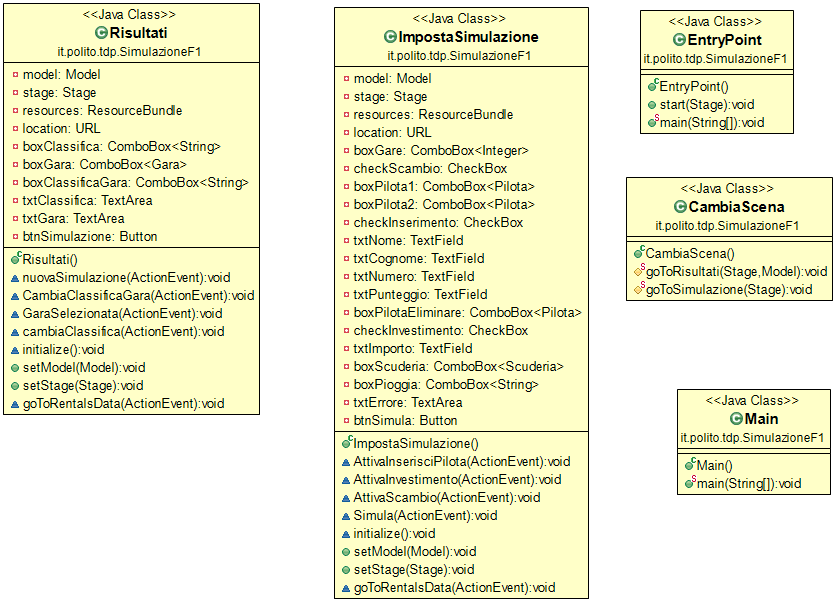
\includegraphics[width=1\linewidth]{images/Diagramma UML package SimulazioneF1.png}
\caption{Diagramma UML package SimulazioneF1}
\label{fig:Diagramma UML package SimulazioneF1}
\end{figure}

\begin{figure}[h]
\centering
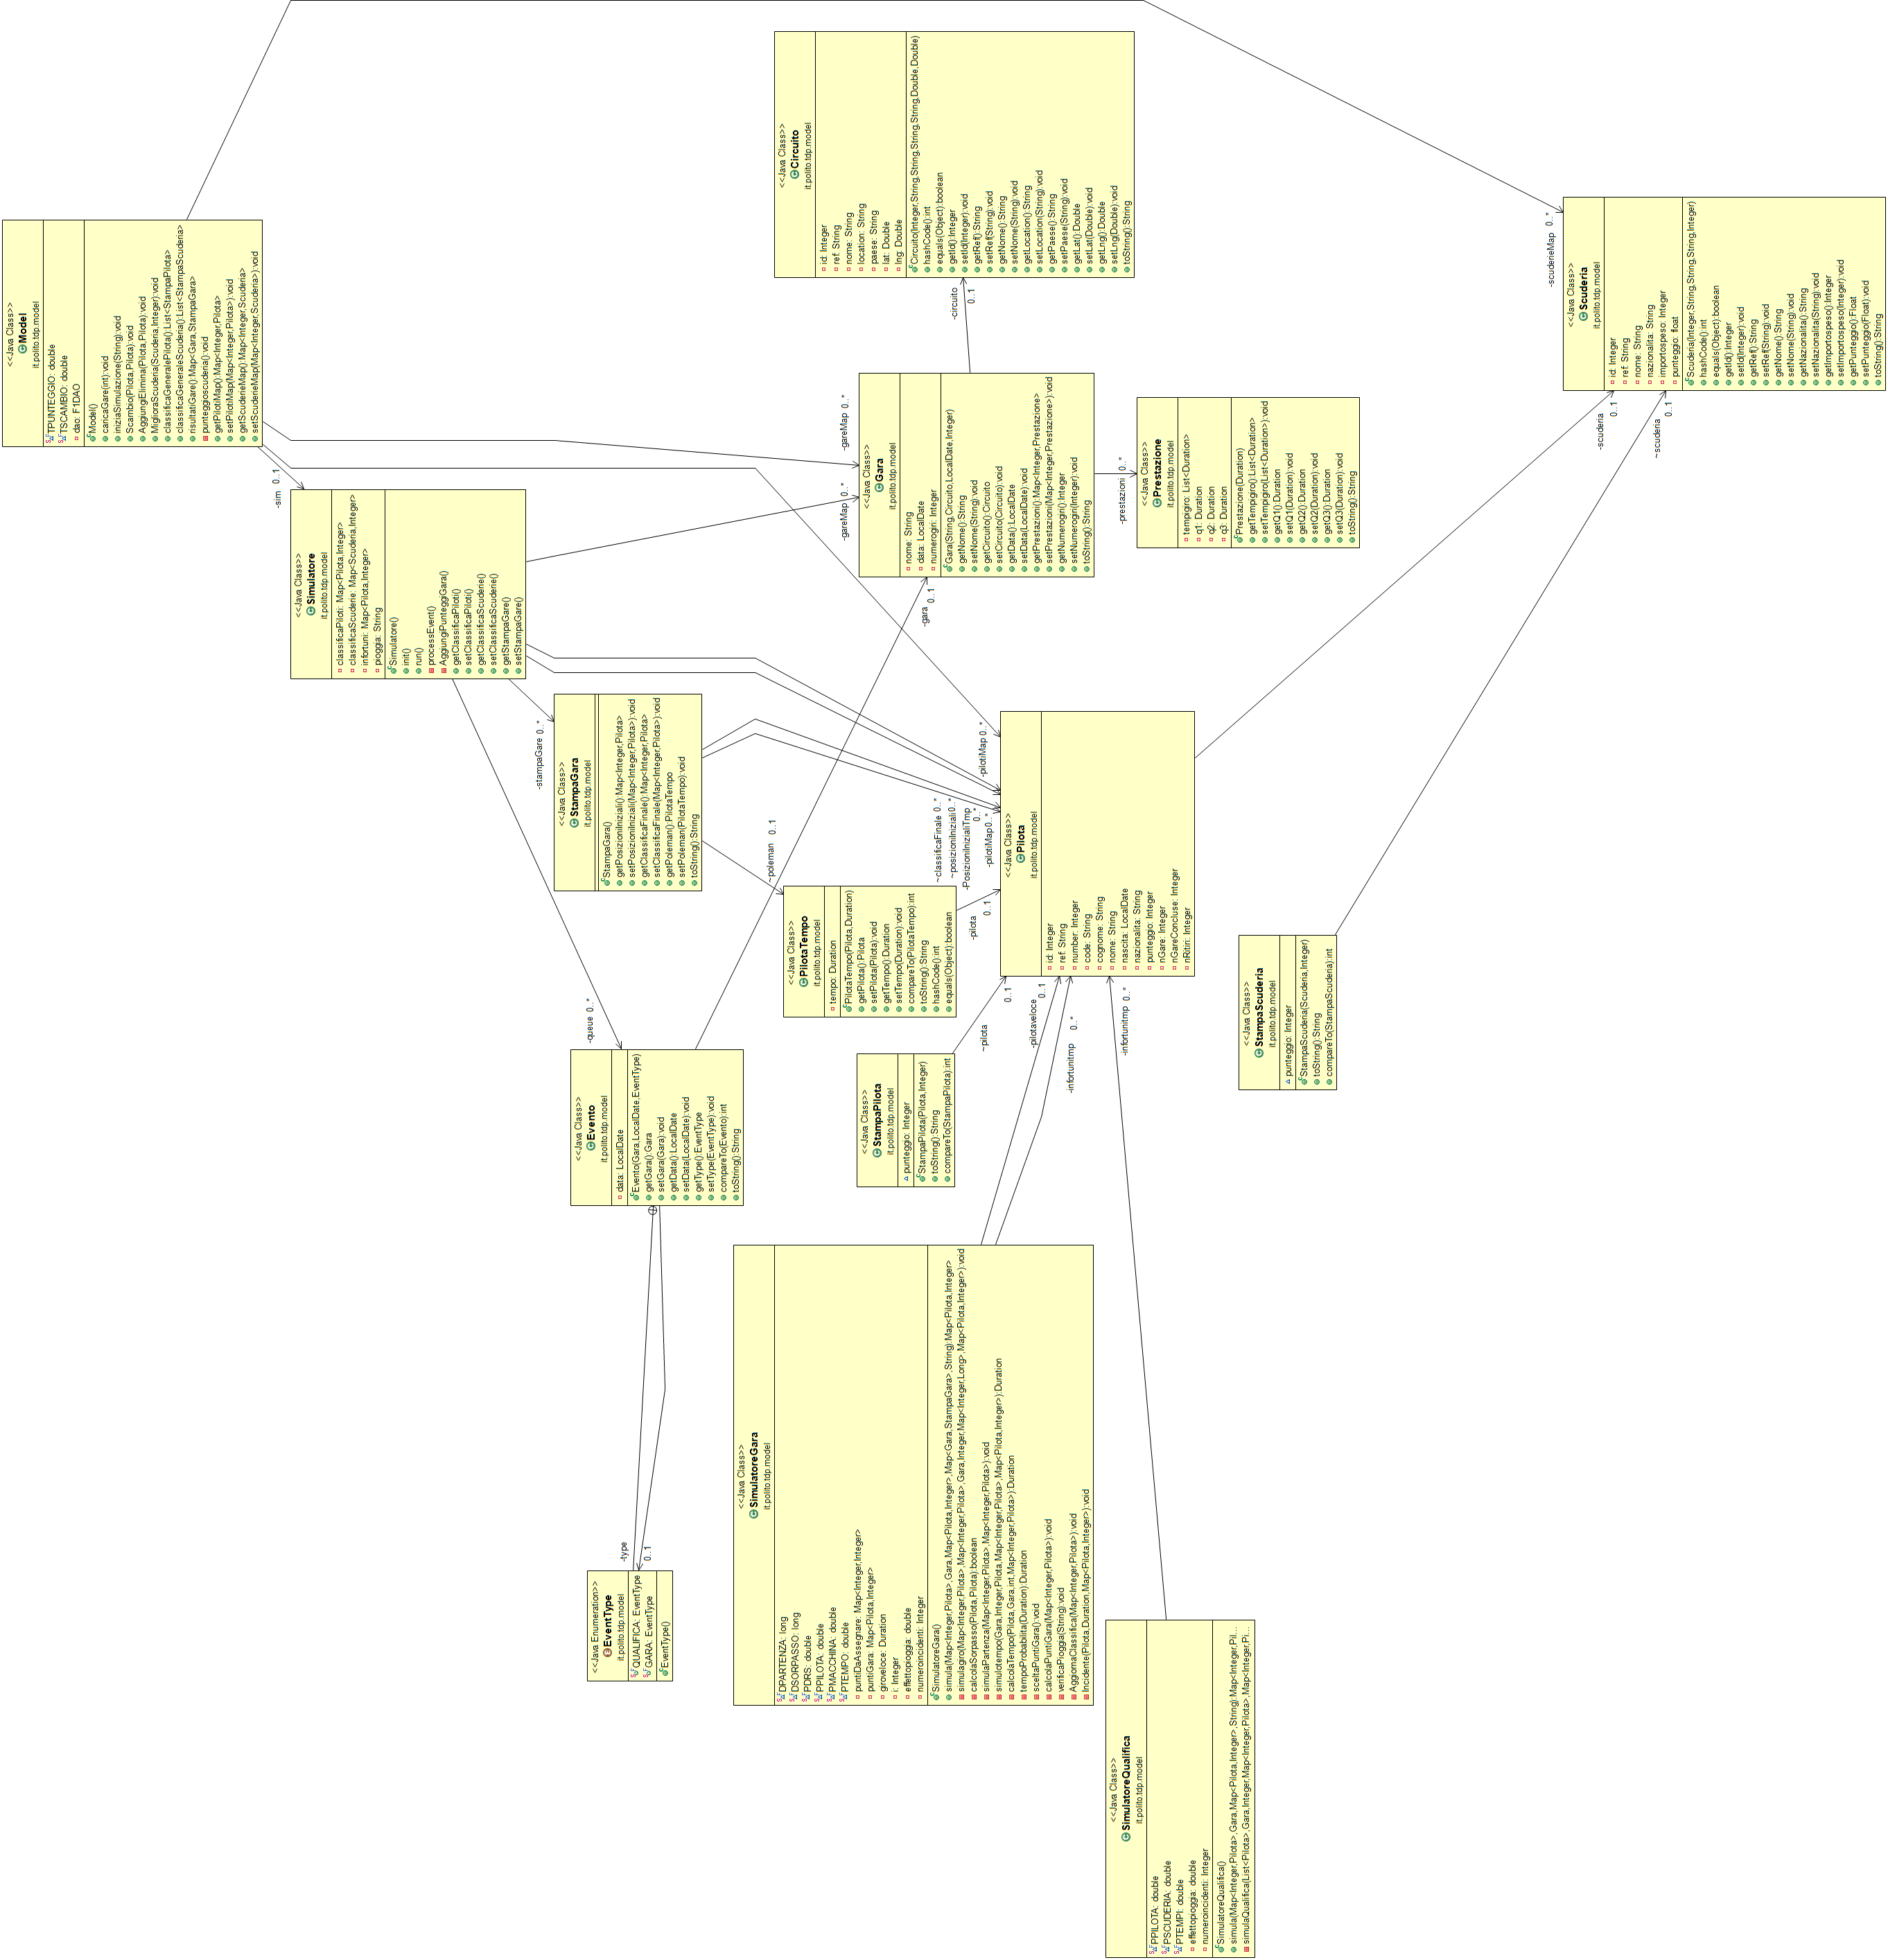
\includegraphics[width=1\linewidth]{images/Diagramma UML package Model2.png}
\caption{Diagramma UML package Model}
\label{fig:Diagramma UML package Model}
\end{figure}

\begin{figure}[h]
\centering
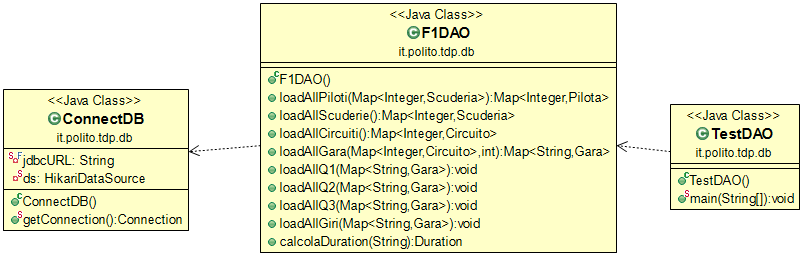
\includegraphics[width=1\linewidth]{images/Diagramma UML package DB.png}
\caption{Diagramma UML package DB}
\label{fig:Diagramma UML package DB}
\end{figure}

\chapter{Interfaccia dell'applicazione}
\label{sec:Interfaccia dell'applicazione}
L'applicazione si compone di 2 schermate, la prima per impostare i dati della simulazione e attraverso il tasto "SIMULA" è possibile passare alla seconda schermata che contiene i risultati della simulazione.

\begin{figure}[h]
\centering
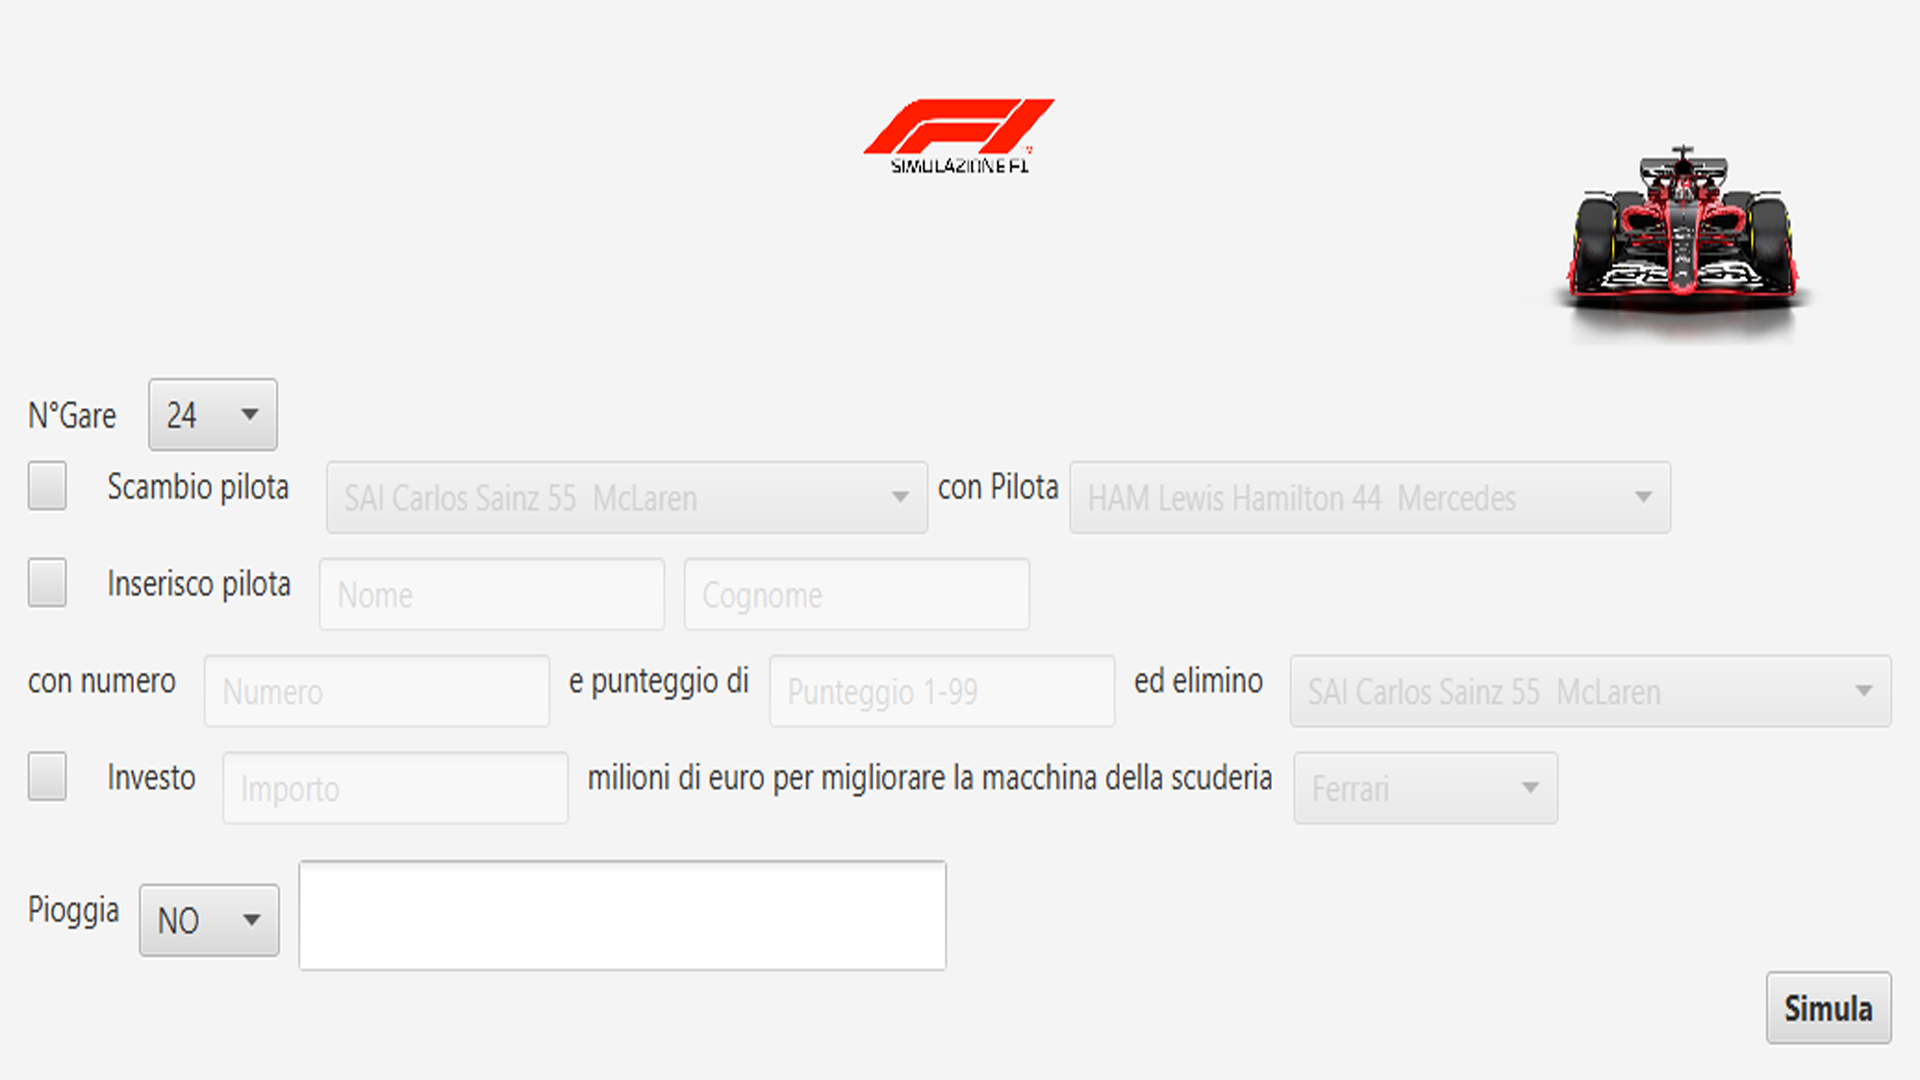
\includegraphics[width=1\linewidth]{images/Schermata impostazione simulazione senza dati.png}
\caption{Schermata impostazione della simulazione}
\label{fig:Schermata impostazione della simulazione}
\end{figure}

\begin{figure}[h]
\centering
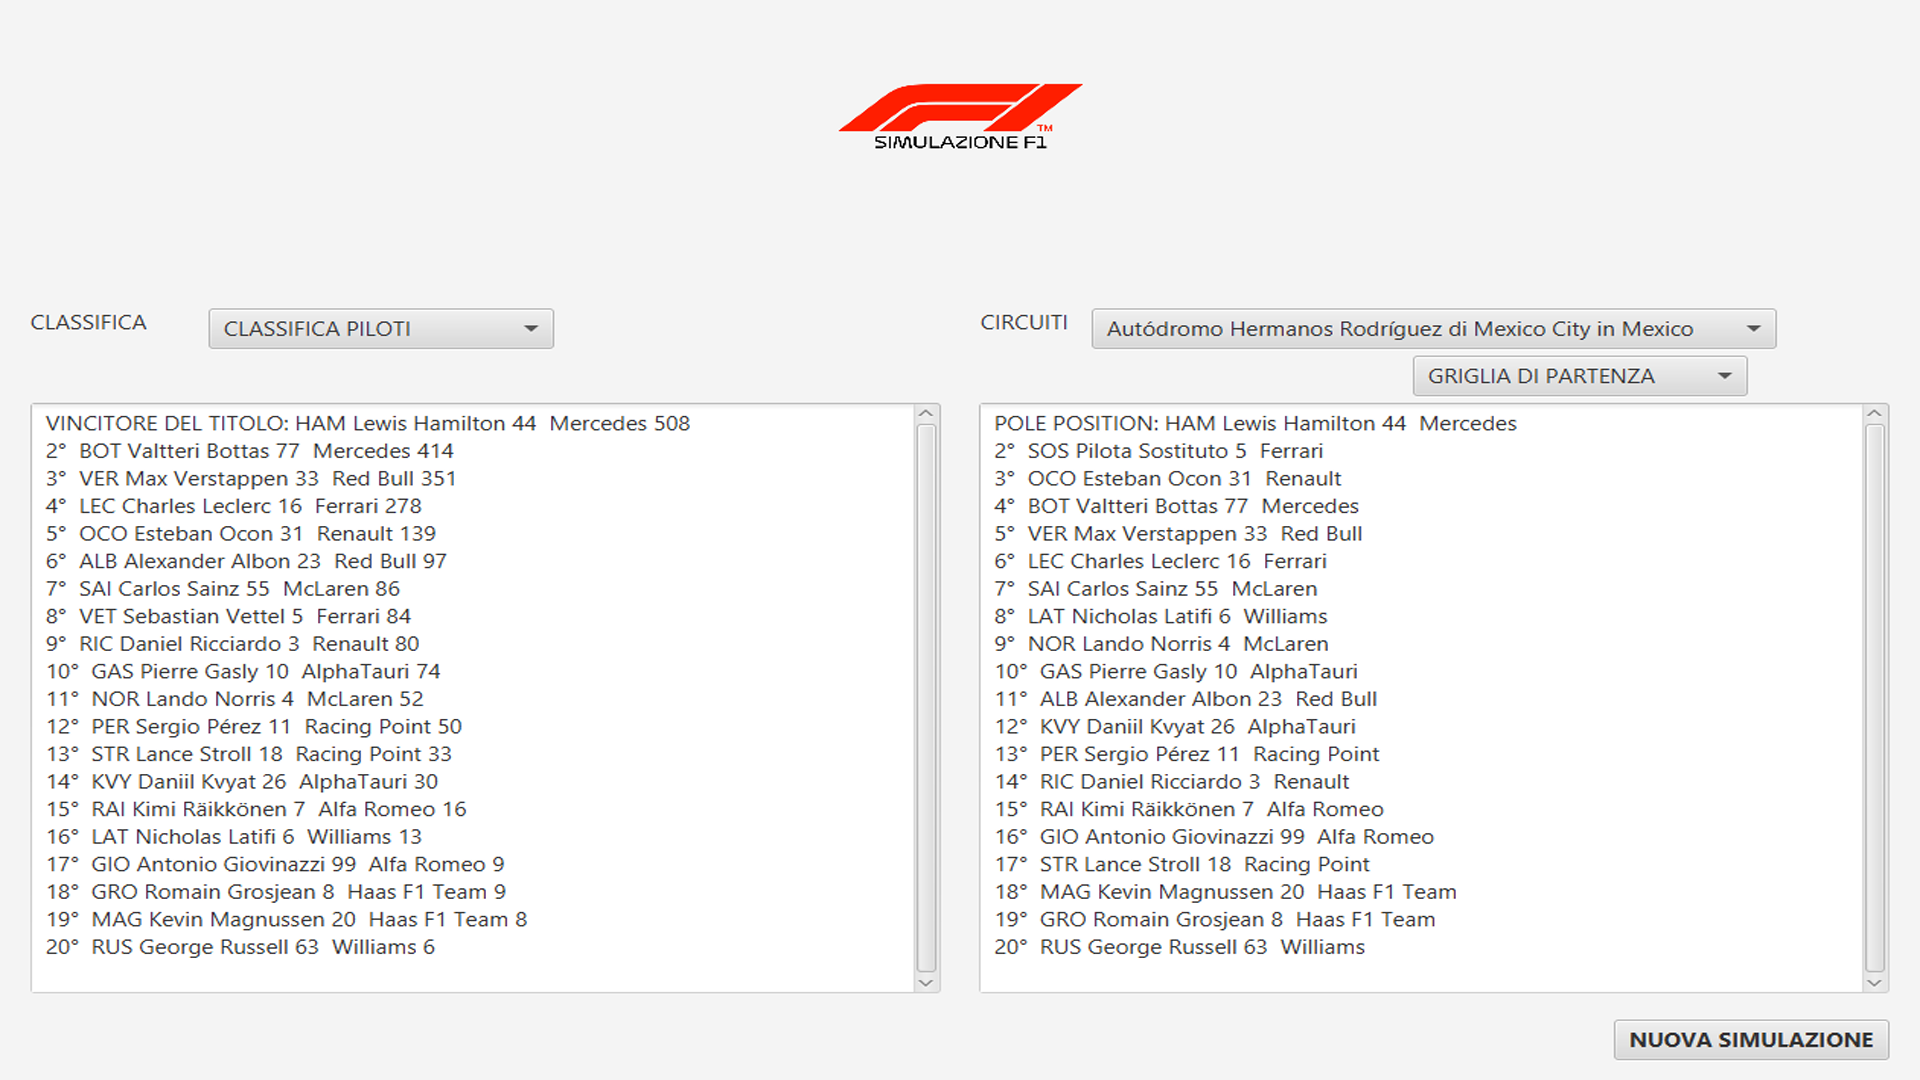
\includegraphics[width=1\linewidth]{images/Risultati piloti.png}
\caption{Classifica Piloti e griglia di partenza della gara in Messico}
\label{fig:Classifica Piloti e griglia di partenza di una gara}
\end{figure}

\begin{figure}[h]
\centering
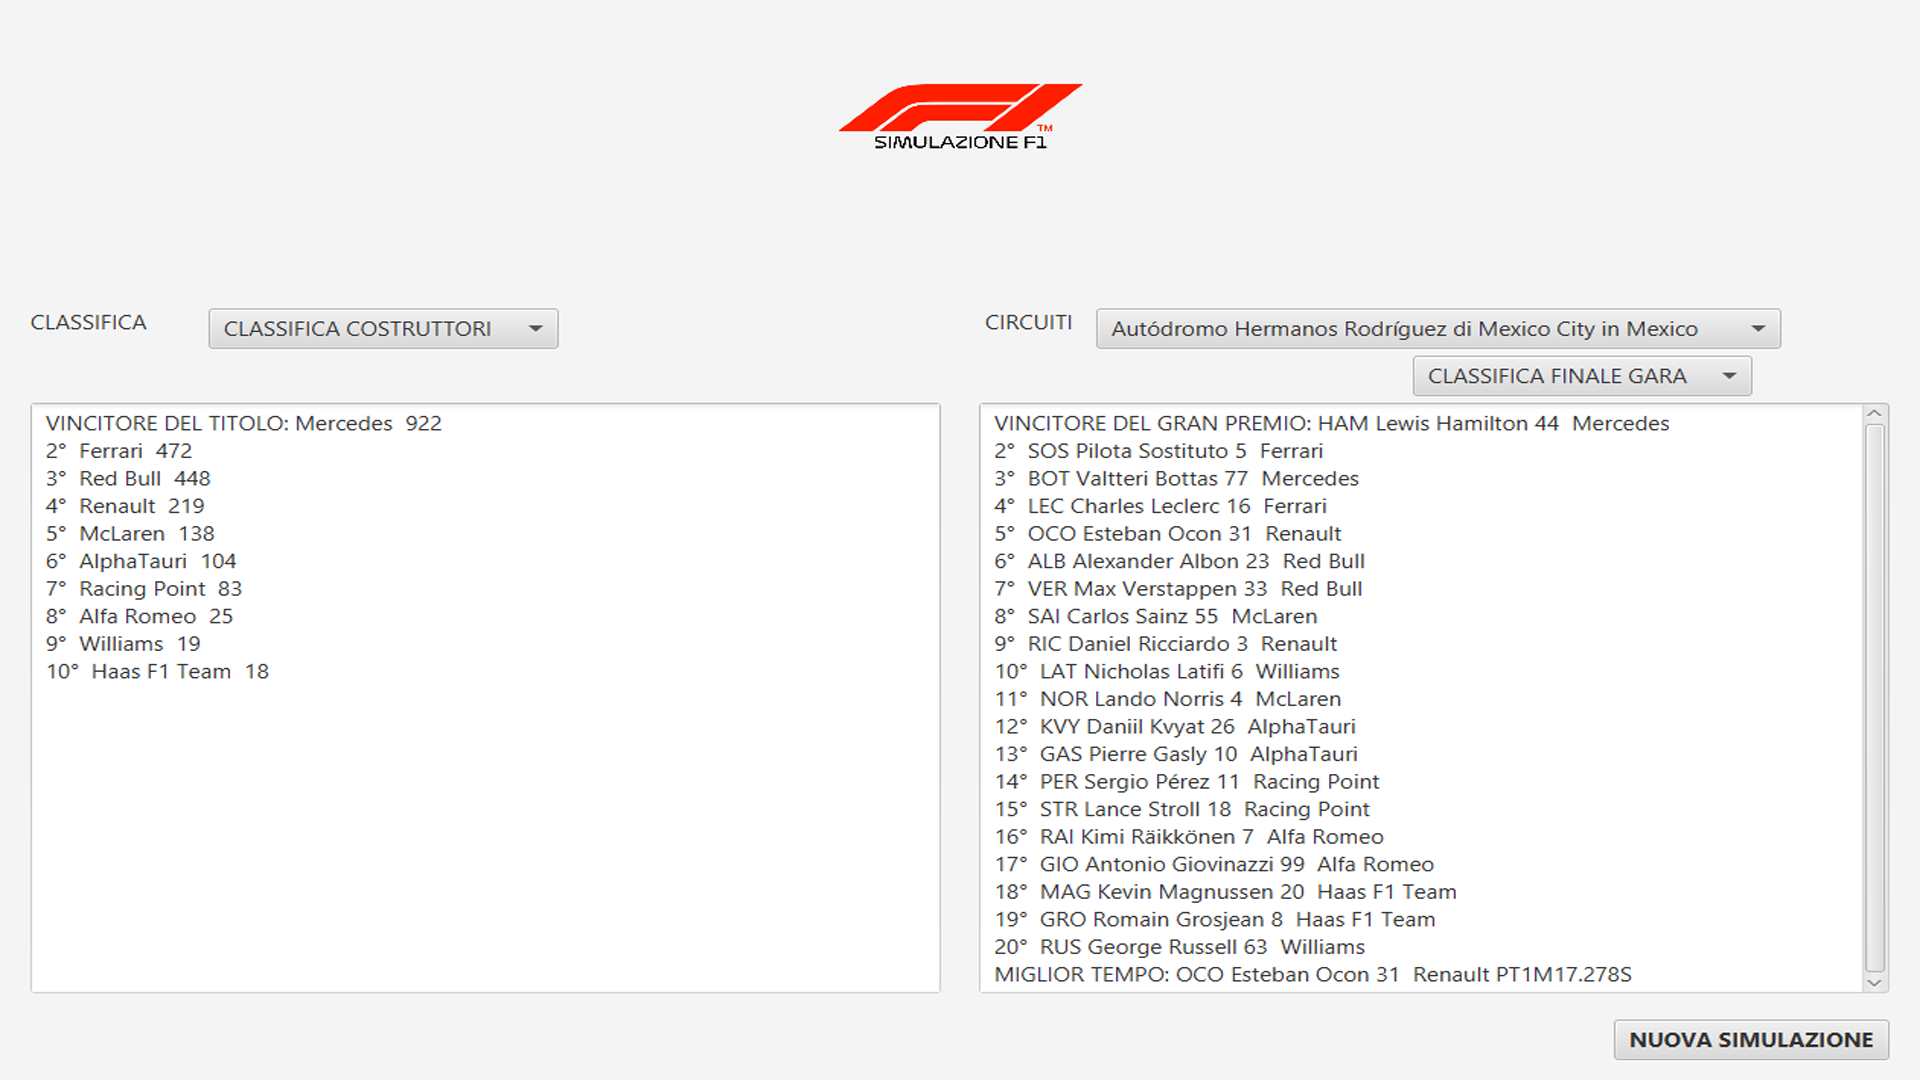
\includegraphics[width=1\linewidth]{images/Risultati scuderia.png}
\caption{Classifica Scuderia e classifica finale della gara in Messico}
\label{fig:Classifica Scuderia e classifica finale di una gara}
\end{figure}

\begin{figure}[h]
\centering
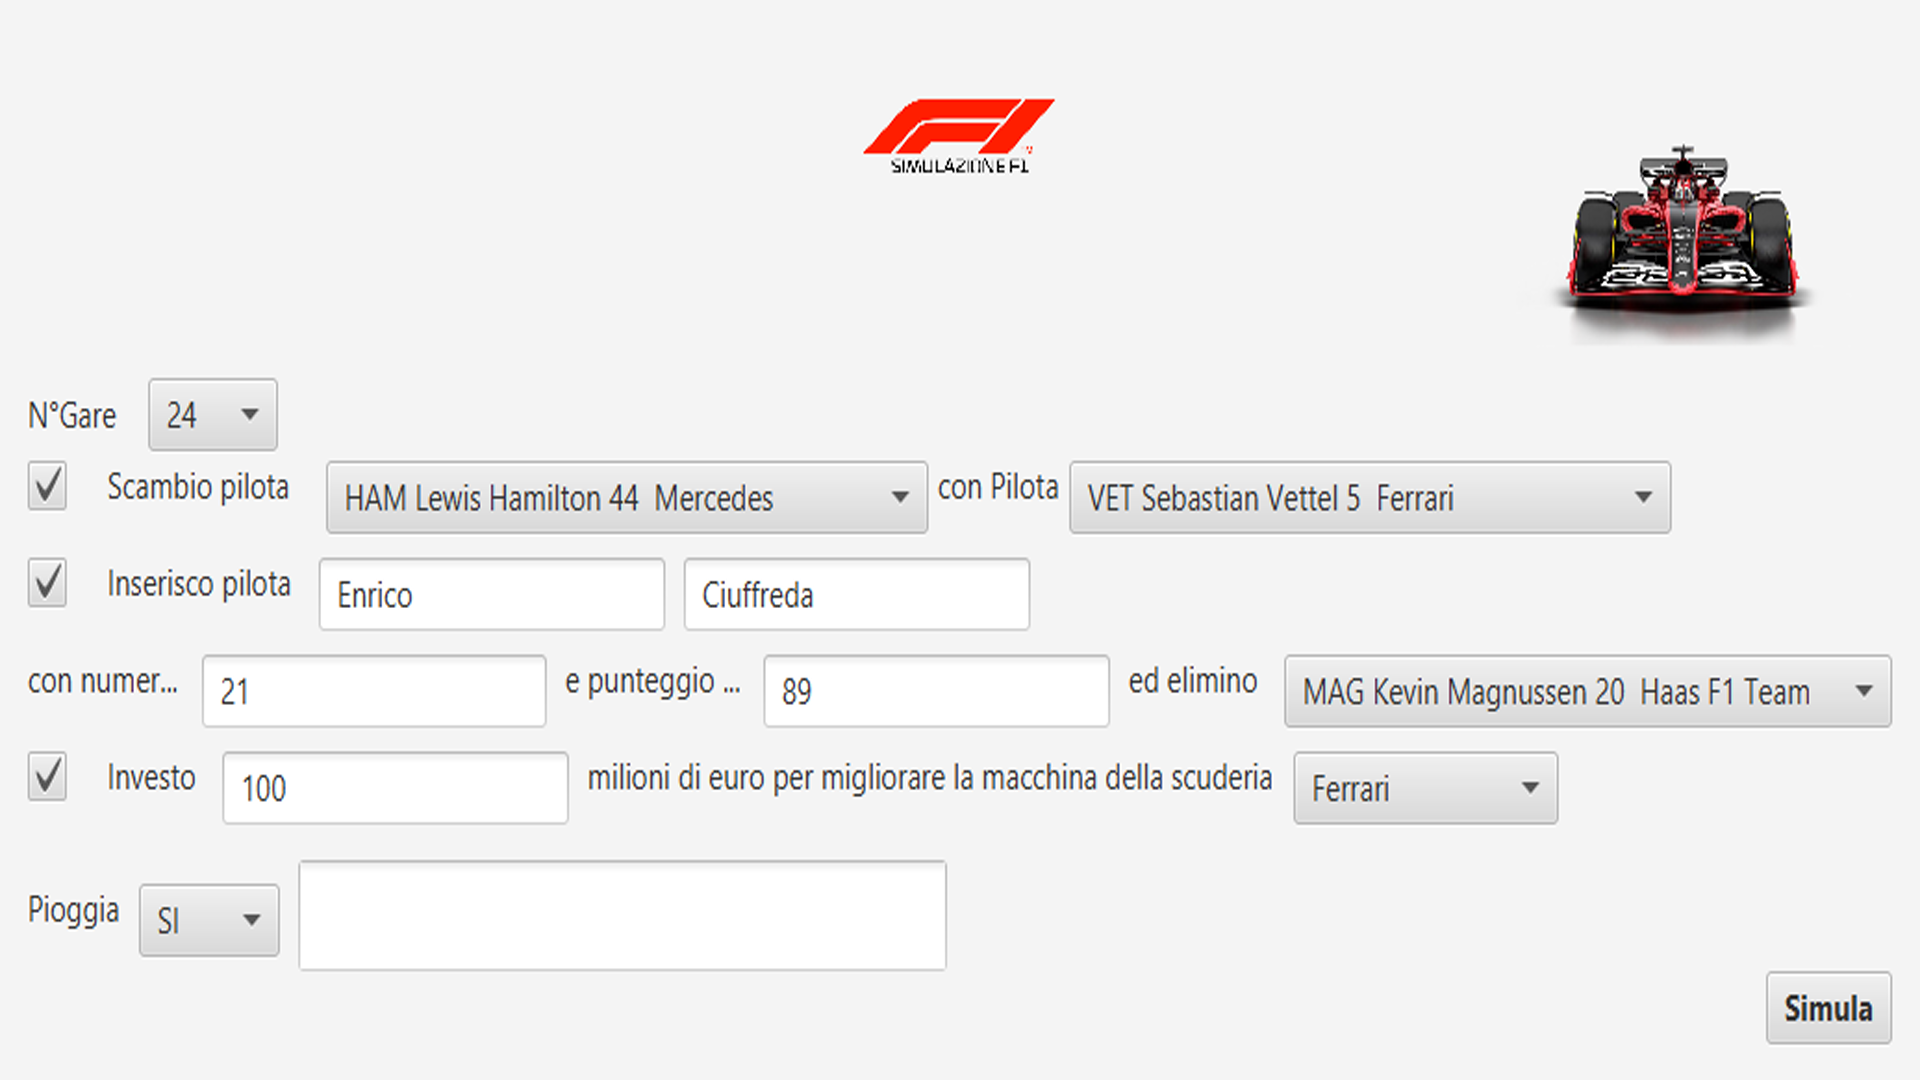
\includegraphics[width=1\linewidth]{images/Schermata impostazione simulazione con dati.png}
\caption{Schermata impostazione della simulazione con dati scelti dall'utente}
\label{fig:Schermata impostazione della simulazione con dati scelti dall'utente}
\end{figure}

\begin{figure}[h]
\centering
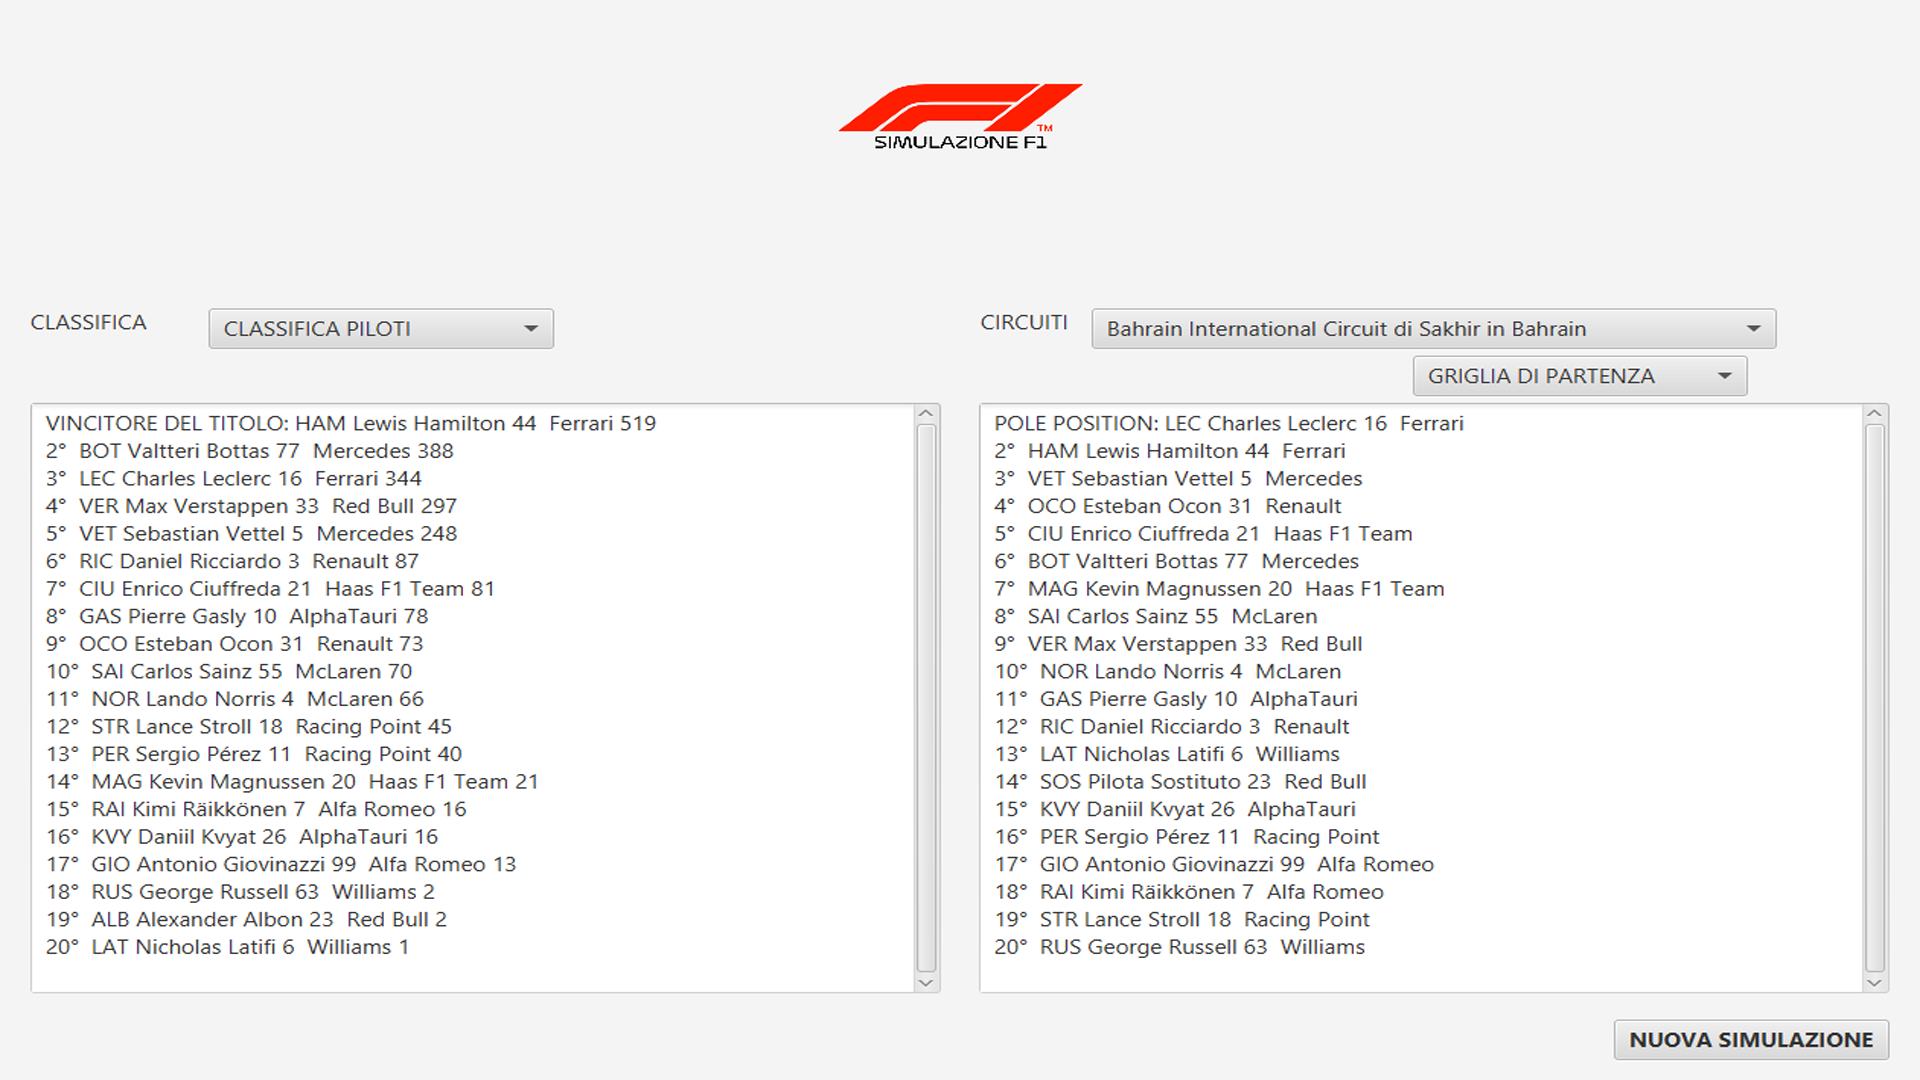
\includegraphics[width=1\linewidth]{images/Risultati ottenuti con impostazioni scelte dall'utente.png}
\caption{Classifica Piloti e griglia di partenza della gara in bahrein}
\label{fig:Classifica Piloti e griglia di partenza di una gara}
\end{figure}

\begin{figure}[h]
\centering
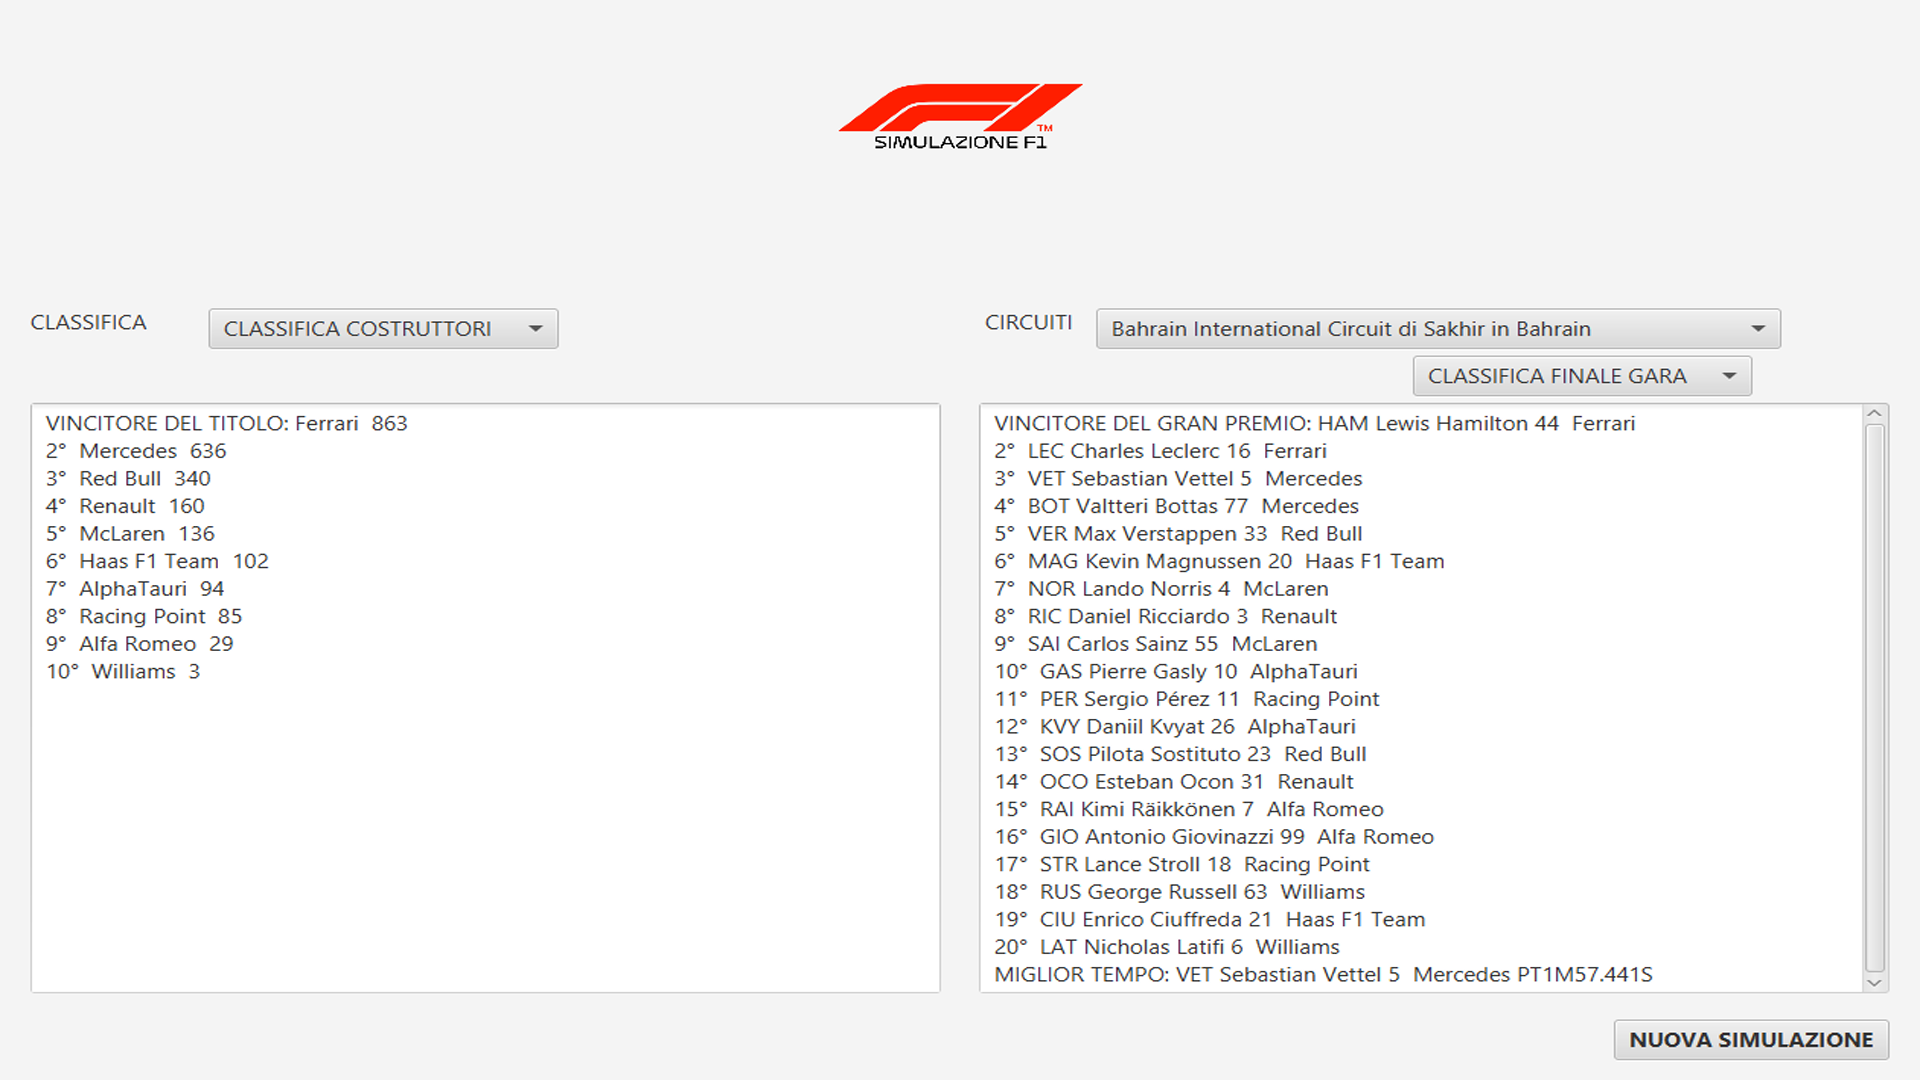
\includegraphics[width=1\linewidth]{images/Risultati scuderia ottenuti con impostazioni scelte dall'utente.png}
\caption{Classifica Scuderia e classifica finale della gara in bahrein}
\label{fig:Classifica Scuderia e classifica finale di una gara}
\end{figure}
\chapter{Esempi d'uso e risultato}
\label{sec:Esempi d'uso e risultato}

\section[Parametri utilizzati]{Parametri utilizzati} % ok with fontsize=12pt
Sono state effettuate cinque diverse simulazione. Le prime tre simulazioni sono state effettuate senza effettuare variazioni. La quarta simulazione è stata effettuata dopo aver scambiato la scuderia di due piloti; il pilota "Lewis Hamilton" della scuderia "Mercedes" è stato scambiato con il pilota "Carlos Sainz" della scuderia "McLaren". La quinta e ultima simulazione è invece stata effettuata dopo aver investito nella scuderia "Ferrari" un quantitativo di milioni di euro pari a trecento.
\begin{figure}[h]
\centering
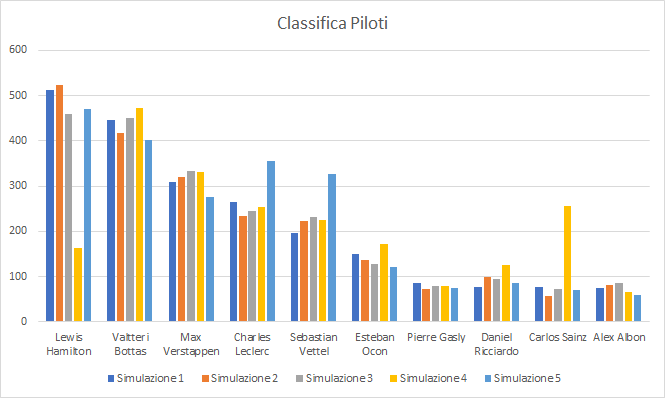
\includegraphics[width=0.9\linewidth]{images/classifica Piloti1.png}
\caption{Classifica Piloti in diverse simulazioni}
\label{fig:Classifica Piloti in diverse simulazioni}
\end{figure}
\begin{figure}[h]
\centering
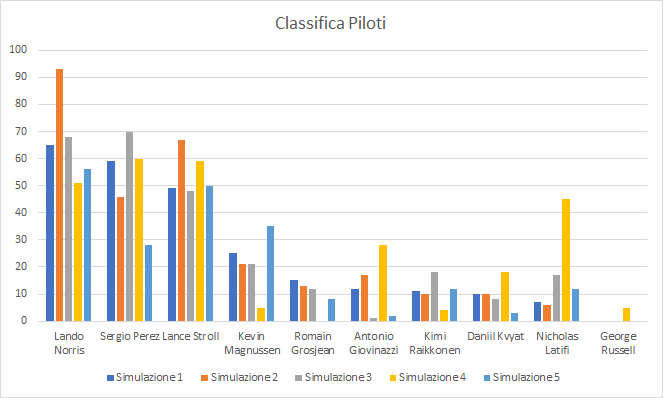
\includegraphics[width=0.9\linewidth]{images/classifica Piloti2.png}
\caption{Classifica Piloti in diverse simulazioni}
\label{fig:Classifica Piloti in diverse simulazioni}
\end{figure}
\begin{figure}[h]
\centering
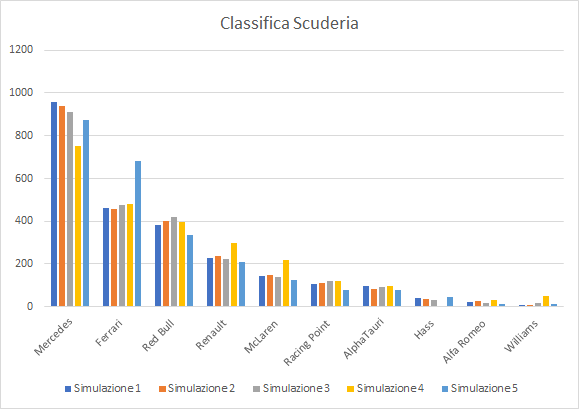
\includegraphics[width=0.9\linewidth]{images/Classifica Scuderia.png}
\caption{Classifica Scuderia in diverse simulazioni}
\label{fig:Classifica Scuderia in diverse simulazioni}
\end{figure}
\clearpage
\section[Analisi]{Analisi} % ok with fontsize=12pt

Dalle figure 7.1, 7.2 e 7.3 è possibile analizzare i risultati delle diverse simulazioni. Come era facilmente pronosticabile il campione del mondo risulta per quattro volte su cinque "Lewis Hamilton" poichè egli ha il punteggio abilità più elevato tra i piloti in griglia, guida la macchina con il punteggio più alto e negli anni precedenti ha ottenuto i migliori tempi. É importante notare che nella figura 7.2 i punteggi dei piloti siano scalati graficamente sul punteggio del pilota che occupa l'undicesima posizione nella prima simulazione. Nella quarta simulazione possiamo osservare gli evidenti effetti di uno scambio di vettura tra due piloti di due scuderie diverse; in questo caso possiamo notare come i due piloti tendano a variare le loro posizioni finali in base alla differenza di punteggio assegnato alle due vetture. Nell'ultima simulazione invece si può vedere come i due piloti della scuderia "Ferrari": "Charles Leclerc" e "Sebastian Vettel" riescano a colmare il gap con "Max Verstappen" ma non il gap con i primi due piloti, entrambi della scuderia "Mercedes"; questo avviene poichè prima della simulazione numero cinque sono stati aumentati i fondi alla scuderia "Ferrari" di un ammontare di milioni pari a trecento e quindi del conseguente miglioramento dei tempi di percorrenza dei giri e del punteggio assegnato alla vettura.\\
Per concludere, una breve riflessione sui dati generati dalle simulazioni. Seppur le simulazioni includono delle variabili aleatorie, i dati che esse producono sono affetti da una notevole dipendenza dei dati delle stagioni passate. Questo si ripercuote sulla poca variabilità delle posizioni finali dei primi classificati; è facilmente intuibile dalle figure 7.2 e 7.3 come la parte centrale della classifica è più affetta a variabilità sia in termini di punteggi finali sia in termini di posizioni questo poichè i punteggi delle vetture, dei piloti e i tempi di giri sono molto vicini tra loro e dunque le variabili casuali tendono a disordinare le posizioni finali dei piloti.
\chapter{Conclusione e possibili miglioramenti}
\label{sec:Conclusione e possibili miglioramenti}

L'applicazione raggiunge tutti gli obiettivi che sono stati previsti in fase di progetto; tuttavia è possibile apportare vari miglioramenti ad essa. Alcuni esempi potrebbero essere l'introduzione di determinati fattori che possono variare i risultati di una gara e di conseguenza anche dell'intero campionato. Tra i vari esempi di fattori non considerati o che potrebbero ottenere un miglioramento possiamo trovare:
\begin{itemize}

    \item\textbf{Abilità del pilota}: questo fattore è stato considerato ma l'abilità è stata valutata attraverso una media di varie abilità possedute dal pilota. Il miglioramento potrebbe consistere nella scissione di questo valore poichè in questa competizione i layout dei vari tracciati delle varie gare sono molto diversi tra loro e questo porterebbe ad una più reale simulazione della gara. 
    \item \textbf{Usura delle gomme}:questo fattore è molto influente in F1 poichè le prestazioni di una vettura in un determinato tracciato dipendono dall'usura degli pneumatici. Questo fattore è stato considerato prendendo come riferimento per il tempo di percorrenza di ogni giro il tempo impiegato da un pilota per percorrere l'iesimo giro e quindi al netto dell'usura delle gomme. Essa,l'usura, potrebbe essere simulata per ogni vettura e ogni pilota poichè anche lo stile di guida potrebbe influenzarla e tutto ciò porterebbe ad una più reale simulazione del campionato;
    \item \textbf{Layout tracciati}: questo fattore non è stato considerato. L'introduzione di questo fattore potrebbe variare in modo significativo la simulazione poichè ogni tracciato prevede ad esempio curve dove vi è un coefficiente di difficoltà di sorpasso molto più alto rispetto a dei rettilinei.\clearpage
    \item \textbf{Strategia Team}: questo fattore potrebbe essere implementato attraverso un algoritmo di machine learning. Un Team-principal decide quali sono le strategie da adottare in gara attraverso l'analisi delle telemetrie, attraverso l'esperienze e attraverso il suo intuito. Eliminando quest'ultima componente, questo lavoro può essere effettuato da una macchina.
\end{itemize}
Infine, soffermandosi ad analizzare i tempi di esecuzione dell'applicazione, si può trarre che la durata della simulazione non sia influenzata notevolmente dal numero idi gare che si decide di far disputare questo poichè si passa da un tempo stimato di circa 45 millisecondi con 24 gare ad un tempo stimato di circa 20 millisecondi con 10 gare; la durata è invece molto influenzata dalla lettura dei dati dal database. Questo accade poichè oltre al tempo di estrazione dei dati, vi è un tempo per elaborare i dati nelle apposite strutture create e il tempo stimato per questo processo è di circa 1 secondo (in media, calcolata su 10 simulazioni, è di 1096 millisecondi). Tenendo conto di queste considerazioni, si ritiene che il margine di miglioramento dei tempi di esecuzione dell'applicazione sia nella possibilità di elaborare query SQL più ottimizzate.

% \paginavuota % it works even without stile=classica
%\ringraziamenti % acknowledgements
%% acknowledgements

ACKNOWLEDGMENTS

\vspace*{5\baselineskip}

\begin{flushright}
    \textit{``HI''\\
    Goofy, \href{https://google.com}{Google} by Google}
\end{flushright}

\clearpage
\thispagestyle{empty}
\null
\vfill
\begin{center}
\doclicenseImage\\
\doclicenseLongText 
\end{center}


% endnotes here if needed

\phantom{0}
\cleardoublepage
\printbibliography[heading=bibintoc] % heading required to show it in ToC

\end{document}
